\documentclass[slidetop,9pt,utf8]{beamer}

\usepackage{CJKutf8}
\usepackage[utf8]{inputenc}
\usepackage[english]{babel}
\usepackage{ifpdf}
\usepackage{textcomp}
\usepackage{color}
\usepackage{xcolor}
\usepackage{amsmath}
\usepackage{graphics}
\usepackage{array}
\usepackage{graphicx}
\usepackage{colortbl}
\usepackage{pinyin}
\usepackage{algorithm,algorithmic}
\usepackage{hyperref}
\usepackage{listingsutf8}
\usepackage{caption}
\usepackage{xspace}

%
%
%  HEADER
%
%

\usetheme{JuanLesPins}
\useoutertheme{infolines}
%\usecolortheme{default}
%\usetheme{Boadilla}
\setbeamerfont{structure}{size*={11}{11}}

\DeclareCaptionFont{white}{\color{white}}
\DeclareCaptionFormat{listing}{\colorbox[cmyk]{0.43, 0.35, 0.35,0.01}{\parbox{\textwidth}{\hspace{15pt}#1#2#3}}}
\captionsetup[lstlisting]{format=listing,labelfont=white,textfont=white, singlelinecheck=false, margin=0pt, font={bf,footnotesize}}

\lstset{
   basicstyle=\footnotesize\ttfamily,
   numberstyle=\tiny,          
   numbersep=5pt,              
   tabsize=2,                  
   extendedchars=true,         
   breaklines=true,            
   keywordstyle=\color{red},
   showspaces=false,           
   showtabs=false,             
   xleftmargin=17pt,
   xrightmargin=17pt,
   framexleftmargin=5pt,
   framexrightmargin=5pt,
   framexbottommargin=4pt,
   showstringspaces=false,
   inputencoding=utf8/latin1      
 }

\lstdefinestyle{terminal}
{
  backgroundcolor=\color{black},
  basicstyle=\scriptsize\color{white}\ttfamily
}

\lstdefinestyle{terminal-large}
{
  backgroundcolor=\color{black},
  basicstyle=\LARGE\color{white}\ttfamily
}

\lstdefinestyle{terminal-medium}
{
  backgroundcolor=\color{black},
  basicstyle=\small\color{white}\ttfamily
}

\lstdefinestyle{code}
{
  frame=b,
  numbers=left,
  morecomment=[is]{/\*}{\*/}
}

% "define" Scala
\lstdefinelanguage{scala}{
  morekeywords={abstract,case,catch,class,def,%
    do,else,extends,false,final,finally,%
    for,if,implicit,import,match,mixin,%
    new,null,object,override,package,%
    private,protected,requires,return,sealed,%
    super,this,throw,trait,true,try,%
    type,val,var,while,with,yield},
  otherkeywords={=>,<-,<\%,<:,>:,\#,@},
  sensitive=true,
  morecomment=[l]{//},
  morecomment=[n]{/*}{*/},
  morestring=[b]",
  morestring=[b]',
  morestring=[b]"""
}

\begin{document}
\begin{CJK}{UTF8}{gbsn}

\AtBeginSection{\frame{\sectionpage}}

\defbeamertemplate{section page}{mine}[1][]{%
  \begin{centering}
    {\usebeamerfont{section name}\usebeamercolor[fg]{section name}#1}
    \begin{beamercolorbox}[sep=12pt,center]{part title}
      \usebeamerfont{section title}\insertsection\par
    \end{beamercolorbox}
  \end{centering}
}

\setbeamertemplate{section page}[mine]

%
%
%  INTRODUCTION
%
%


%--- title page ---
\title[Spark Hands On (PSUG)]{Spark Hands On}
\subtitle{Paris Scala User Group}
\author{Olivier GIRARDOT, Vincent DOBA}
\institute[LT]{Lateral-Thoughts}
\date{May 13, 2015}

\frame{\titlepage}

%--- Summary ---
\begin{frame}[allowframebreaks]
  \frametitle{Content}
  \tableofcontents[hideallsubsections]
\end{frame}

\section{Prerequisite}

%--- Prerequisite for the machine ---
\begin{frame}
  \frametitle{Machine Prerequisite}

  \begin{block}{You should have}
    \begin{itemize}
      \item JDK 7+ (this hands on was developed using Oracle JDK 8) with Scala 2.10+
      \item SBT 13+
      \item Git
      \item An IDE with SBT/Scala support (for instance IDEA IntelliJ with SBT and Scala plugins)
      \item \textbf{For Exercise 9} Downloaded Spark 1.3.1 prebuilt for Hadoop 2.6 from \href{http://www.apache.org/dyn/closer.cgi/spark/spark-1.3.1/spark-1.3.1-bin-hadoop2.6.tgz}{official Apache Spark site}
    \end{itemize}
  \end{block}

  \begin{block}{You should know}
    \begin{itemize}
      \item Scala basis (functions, val, pattern matching)
      \item Scala iterables transformations (map, flatmap, fold)
      \item Anonymous functions
    \end{itemize}
  \end{block}

\end{frame}

%--- First Spark Run
\begin{frame}[fragile]
  \frametitle{First Spark Run}

  \begin{block}{Perform following commands}
    \begin{lstlisting}[language=bash, style=terminal-medium]
git clone https://github.com/vincentdoba/spark-hands-on.git
cd spark-hands-on
sbt "run-main psug.hands.on.prerequisite.WordCount README.md" 
    \end{lstlisting}
  \end{block}

  \begin{block}{You should obtain}
    \begin{lstlisting}[language=bash, style=terminal]
[info] Running psug.hands.on.prerequisite.WordCount README.md
[error] 15/05/08 17:37:36 WARN NativeCodeLoader: Unable to load native-hadoop library for your platform... using builtin-java classes where applicable
[info] (,48)
[info] (*,24)
[info] (####,16)
[info] (of,14)
[info] (the,11)
[info] (###,10)
[info] (Exercise,8)
[info] (Description,8)
[info] (Notions,8)
[info] (a,8)
[success] Total time: 25 s, completed 8 mai 2015 17:37:39
    \end{lstlisting}
  \end{block}

%--- World Count Script ---
\end{frame}

\begin{frame}[fragile]
  \frametitle{Words Count Script}

  \lstinputlisting[language=scala, style=code, label=WordCount,caption=/src/main/scala/psug/hands/on/prerequisite/WordCount.scala]{../src/main/scala/psug/hands/on/prerequisite/WordCount.scala}

\end{frame}

%--- Important Notions (1) ---
\begin{frame}
  \frametitle{Important Notions (1)}

  \begin{block}{Vocabulary}
    \begin{itemize}
      \item \textbf{Spark Conf} Configuration of the Spark Context, here contains application name and master to call
      \item \textbf{Spark Context} Main entry point, represents the connection to a Spark Cluster, used to create RDDs/Load file
      \item \textbf{Resilient Distribued Dataset (RDD)} Main Dataset abstraction on which we can apply actions and transformations
      \item \textbf{Transformations} functions that transform RDD to another RDD
      \item \textbf{Actions} functions that transform a RDD to output data
    \end{itemize}
  \end{block}

\end{frame}

%--- Important Notions (2) ---
\begin{frame}
  \frametitle{Important Notions (2)}

  \begin{block}{Spark Scripting How To}
    \begin{itemize}
      \item Initiate a Spark Context
      \item Load a dataset into a RDD thanks to the Spark Context
      \item Register Transformations on RDD
      \item Apply an Action to transformed RDD
      \item Stop Spark Context
      \item Do whatever you want with data obtained after 
    \end{itemize}
  \end{block}

\end{frame}

%--- SBT Configuration ---
\begin{frame}
  \frametitle{SBT Configuration}

  \lstinputlisting[language=scala, style=code, label=SbtBuild,caption=/build.sbt]{../build.sbt}

\end{frame}

%--- Log4J Configuration ---
\begin{frame}
  \frametitle{Log4J Configuration}

  \lstinputlisting[language=java, style=code, label=log4j,caption=/src/main/resources/log4j.properties]{../src/main/resources/log4j.properties}

\end{frame}

%
%
%  EXERCISE 1
%
%

\section{Exercise 1 : Spark basis (SparkContext, RDD, Transformation, Action)}


%--- Exercise 1 ---
\begin{frame}
  \frametitle{Exercise 1}

  \begin{block}{Statement}
    We have three lists : 
    \begin{itemize}
      \item First list contains the integers from 1 to 75
      \item Second list contains the integers from 25 to 100
      \item Third list contains primes under 100. 
    \end{itemize}
    We want to obtain the sum of square of integers that are under 100 and are not prime.
    \\ \medskip
    For instance, the sum of square of intergers that are under 10 and are not prime is
    $1^{2} + 4^{2} + 6^{2} + 8^{2} + 9^{2} + 10^{2} = 298$
  \end{block}

  \begin{block}{What you will learn}
    \begin{itemize}
      \item Initialization of Spark Context
      \item Transform Scala lists to Spark RDDs
      \item Discover some transformations on RDDs
      \item Discover first action : reduce
    \end{itemize}
  \end{block}

\end{frame}

%--- EX1 : Exercise code ---
\begin{frame}
  \frametitle{Exercise Code}

  \lstinputlisting[language=scala, style=code, label=Exercise1,caption=/src/main/scala/psug/hands/on/exercise01/SumOfSquareOfNonPrimeNumbers.scala]{../src/main/scala/psug/hands/on/exercise01/SumOfSquareOfNonPrimeNumbers.scala}

\end{frame}

%--- EX1 : New Notions (1) ---
\begin{frame}[fragile]
  \frametitle{New Notions (1)}

  \begin{lstlisting}[label=InitSparkContext, caption=Init Spark Context, language=scala, style=code]
val conf = new SparkConf()
  .setMaster("local")
  .setAppName("applicationName")
val sparkContext = new SparkContext(conf)
  \end{lstlisting}

  \begin{lstlisting}[label=ListToRdd, caption=Load List as RDD, language=scala, style=code]
val scalaList:List[T] = List(...)
val rdd1:RDD[T] = sparkContext.makeRDD(scalaList)
val rdd2:RDD[T] = sparkContext.parallelize(scalaList) // exactly same thing
  \end{lstlisting}

\end{frame}

%--- EX1 : New Notions (2) ---
\begin{frame}[fragile]
  \frametitle{New Notions (2)}

  \begin{lstlisting}[label=RDDTransformation, caption=Apply transformation to RDD, language=scala, style=code]
val newRdd:RDD[T] = oldRdd.map(x => x)
  \end{lstlisting}

  \begin{lstlisting}[label=RDDAction, caption=Apply action to RDD, language=scala, style=code]
val result:T = rdd[T].reduce((a,b) => f(a,b))
  \end{lstlisting}

  \begin{lstlisting}[label=StopSparkContext, caption=Stop Spark Context, language=scala, style=code]
sparkContext.stop()
  \end{lstlisting}

\end{frame}

%--- EX1 : New Transformations and Actions
\begin{frame}

  \frametitle{New Transformations and Actions}

  \begin{block}{Transformations}
    \begin{center}
      \begin{tabular}{|m{2.1cm}|m{3.5cm}|m{5cm}|}
        \hline 
        \rowcolor{gray} \textbf{Transformation} & \textbf{Usage} & \textbf{Description} \\ \hline
        \textbf{union} & \textit{rdd1.union(rdd2)} & merge the two rdds \\ \hline
        \textbf{distinct} & \textit{rdd1.distinct()} & remove duplicates from rdd \\ \hline
        \textbf{subtract} & \textit{rdd1.substract(rdd2)} & remove values from rdd2 of rdd1 \\ \hline
        \textbf{map} & \textit{rdd1.map(f: (T) =\textgreater\xspace U)} & apply function f to elements of rdd1 \\ \hline
      \end{tabular}
    \end{center}
  \end{block}

  \begin{block}{Actions}
    \begin{center}
      \begin{tabular}{|m{2.1cm}|m{3.5cm}|m{5cm}|}
        \hline 
        \rowcolor{gray} \textbf{Action} & \textbf{Usage} & \textbf{Description} \\ \hline
        \textbf{reduce} & \textit{rdd1[T].reduce(f(T,T) =\textgreater\xspace T)} & merge 2 by 2 the elements of RDD using function f to one element \\ \hline
      \end{tabular}
    \end{center}
  \end{block}

\end{frame}

%--- EX1 : Run ---
\begin{frame}[fragile]
  \frametitle{Command and Result}

  \begin{block}{Command}
    \begin{lstlisting}[language=bash, style=terminal-medium]
sbt "run-main psug.hands.on.exercise01.SumOfSquaresOfNonPrimeNumbers"
    \end{lstlisting}
  \end{block}

  \begin{block}{Result}
    \begin{lstlisting}[language=bash, style=terminal]
[info] The sum of square of numbers that are not prime and are under 100 is 272554.0
[success] Total time: 9 s, completed 8 mai 2015 21:23:22
    \end{lstlisting}
  \end{block}

\end{frame}

%--- EX1 : Notes
\begin{frame}
  \frametitle{Notes}

  \begin{exampleblock}{Transformation/Action}
    \begin{itemize}
      \item A RDD doesn't contain the data, it is a representation of the data (Abstraction of a data set)
      \item When you declare transformations on a RDD, these transformations are not resolved yet (Lazyness)
      \item It is when you call an action that the data are loaded and transformations are resolved
    \end{itemize}
  \end{exampleblock}

\end{frame}

%
%
%  EXERCISE 2
%
%

\section{Exercise 2 : Key/Values RDD, File Loading}


%--- Exercise 2 ---
\begin{frame}
  \frametitle{Exercise 2}

  \begin{block}{Statement}
    We have a text file containing the list of French departments. Which are the departments whose name contains Seine ? And Loire ? And Garonne ? And Rhône ?
  \end{block}

  \begin{block}{What you will learn}
    \begin{itemize}
      \item Load a file using a Spark Context
      \item New Actions and Transformations
      \item How to transform an RDD to a Key/Value RDD
    \end{itemize}
  \end{block}

\end{frame}

%--- EX2 : Exercise Code ---
\begin{frame}
  \frametitle{Exercise Code}

  \lstinputlisting[language=scala, style=code, label=Exercise2,caption=/src/main/scala/psug/hands/on/exercise02/DepartmentsByRiver.scala]{../src/main/scala/psug/hands/on/exercise02/DepartmentsByRiver.scala}

\end{frame}

%--- EX2 : Input Description ---
\begin{frame}[fragile]
  \frametitle{departements.txt File}

  \begin{verbatim}
Ain,01
Aisne,02
Allier,03
Alpes-de-Haute-Provence,04
Hautes-Alpes,05
Alpes-Maritimes,06
Ardèche,07
Ardennes,08
Ariège,09
Aube,10
Aude,11
Aveyron,12
Bouches-du-Rhône,13
Calvados,14
Cantal,15
Charente,16
Charente-Maritime,17
...
  \end{verbatim}

\end{frame}

%--- EX2 : New Notions ---
\begin{frame}[fragile]
  \frametitle{New Notions}

  \begin{lstlisting}[label=LoadTextFile, caption=Load Text File, language=scala, style=code]
val rdd:RDD[String] = sparkContext.textFile("filePath")
  \end{lstlisting}

  \begin{lstlisting}[label=TransformToKeyValue, caption=Transform RDD to a Key/Value RDD (Also called PairRDD), language=scala, style=code]
val keyValueRdd1:RDD[(K,V)] = oldRdd[T].map(f: (T) => (K,V))
val keyValueRdd2:RDD[(K,V)] = oldRdd[T]
  .flatMap(f: (T) => TraversableOnce[(K,V)])
  \end{lstlisting}

\end{frame}

%--- EX2 : New Transformations and Actions ---
\begin{frame}

  \frametitle{New Transformations and Actions}

  \begin{block}{Transformations}
    \begin{center}
      \begin{tabular}{|m{2.0cm}|m{4.0cm}|m{4.9cm}|}
        \hline 
        \rowcolor{gray} \textbf{Transformation} & \textbf{Usage} & \textbf{Description} \\ \hline
        \textbf{filter} & \textit{rdd1[T]\newline.filter(f: (T) =\textgreater\xspace boolean)} & filter by function f \\ \hline
        \textbf{flatMap} & \textit{rdd1[T].flatMap(f: (T) =\textgreater\xspace TraversableOnce[U])} & apply function f and flatten \\ \hline
        \textbf{reduceByKey} & \textit{rdd1[(K,V)]\newline.reduceByKey(f:(V,V) =\textgreater\xspace V)} & create an RDD containing tuples (K, V), unique by key \\ \hline
        \textbf{sortByKey} & \textit{rdd1[(K,V)].sortByKey()} & sort rdd1 by key \\ \hline
      \end{tabular}
    \end{center}
  \end{block}

  \begin{block}{Actions}
    \begin{center}
      \begin{tabular}{|m{2.0cm}|m{4.0cm}|m{4.9cm}|}
        \hline 
        \rowcolor{gray} \textbf{Action} & \textbf{Usage} & \textbf{Description} \\ \hline
        \textbf{collect} & \textit{rdd1.collect()} & retrieve all elements of RDD as Array \\ \hline
      \end{tabular}
    \end{center}
  \end{block}

\end{frame}

%--- EX2 : Run ---
\begin{frame}[fragile]
  \frametitle{Command and Result}

  \begin{block}{Command}
    \begin{lstlisting}[language=bash, style=terminal-medium]
sbt "run-main psug.hands.on.exercise02.DepartmentsByRiver"
    \end{lstlisting}
  \end{block}

  \begin{block}{Result}
    \begin{lstlisting}[language=bash, style=terminal]
[info] Les departements dont le nom contient Garonne sont Haute-Garonne, Lot-et-Garonne, Tarn-et-Garonne
[info] Les departements dont le nom contient Loire sont Indre-et-Loire, Loire, Haute-Loire, Loire-Atlantique, Loiret, Maine-et-Loire, Saone-et-Loire
[info] Les departements dont le nom contient Rhone sont Bouches-du-Rhone, Rhone
[info] Les departements dont le nom contient Seine sont Seine-Maritime, Seine-et-Marne, Hauts-de-Seine, Seine-Saint-Denis
[success] Total time: 8 s, completed 8 mai 2015 22:03:26
    \end{lstlisting}
  \end{block}

\end{frame}

%--- EX2 : Notes ---
\begin{frame}
  \frametitle{Notes}

  \begin{exampleblock}{Collect/Foreach}
    \begin{itemize}
      \item In this Exercise, we used \textit{collect} action to retrieve all elements of RDD and then print them using \textit{foreach} scala iterable's method
      \item Except if there are few elements at the end of RDD transformations, it is not a good idea to call \textit{collect}
      \item Here, we could have directly used \textit{foreach} action that is more efficient
    \end{itemize}
  \end{exampleblock}

  \begin{exampleblock}{GroupByKey}
    \begin{itemize}
      \item \textit{GroupByKey} transformation transform a RDD[K,V] to a RDD[K, Iterable[V]], iterable containing all the values under that key
      \item Meaning when you use it on large data set, there is lot of data transferred
      \item It should be avoided and replaced by \textit{reduceByKey} transformation
    \end{itemize}
  \end{exampleblock}

\end{frame}

%
%
% EXERCISE 3
%
%

\section{Exercise 3 : Spark SQL Context, JSON Loading, DataFrames}

%--- Exercise 3 ---
\begin{frame}
  \frametitle{Exercise 3}

  \begin{block}{Statement}
    We have a JSON file containing the list of French cities with population. What is the total population of France ?
  \end{block}

  \begin{block}{What you will learn}
    \begin{itemize}
      \item Initialize Spark SQL Context
      \item Load DataFrames from JSON File with a Spark SQL Context
      \item First Actions and Transformations on DataFrames
    \end{itemize}
  \end{block}

\end{frame}

%--- EX3 : Exercise Code ---
\begin{frame}
  \frametitle{Exercise Code}

  \lstinputlisting[language=scala, style=code, label=Exercise3,caption=/src/main/scala/psug/hands/on/exercise03/TotalPopulation.scala]{../src/main/scala/psug/hands/on/exercise03/TotalPopulation.scala}

\end{frame}

%--- EX3 : Input ---
\begin{frame}[fragile]
  \frametitle{demographie\_par\_commune.json File}

  \begin{verbatim}
{"CodeInsee":"01001",[...],"Population":784,[...]}
{"CodeInsee":"01002",[...],"Population":221,[...]}
{"CodeInsee":"01004",[...],"Population":13835,[...]}
{"CodeInsee":"01005",[...],"Population":1616,[...]}
{"CodeInsee":"01006",[...],"Population":116,[...]}
{"CodeInsee":"01007",[...],"Population":2362,[...]}
{"CodeInsee":"01008",[...],"Population":729,[...]}
{"CodeInsee":"01009",[...],"Population":340,[...]}
{"CodeInsee":"01010",[...],"Population":994,[...]}
{"CodeInsee":"01011",[...],"Population":363,[...]}
{"CodeInsee":"01012",[...],"Population":302,[...]}
{"CodeInsee":"01013",[...],"Population":163,[...]}
{"CodeInsee":"01014",[...],"Population":3476,[...]}
{"CodeInsee":"01015",[...],"Population":480,[...]}
{"CodeInsee":"01016",[...],"Population":399,[...]}
{"CodeInsee":"01017",[...],"Population":421,[...]}
{"CodeInsee":"01019",[...],"Population":20,[...]}
...
  \end{verbatim}
\end{frame}

%--- EX3 : New Notions (1) ---
\begin{frame}
  \frametitle{New Notions (1)}

  \begin{block}{Data Frame}
    \begin{itemize}
      \item Equivalent of RDD for structured data, DataFrame class extends RDD Api
      \item Can be seen as a SQL Table (columns and set of rows)
      \item Has specific Transformations/Actions
    \end{itemize}
  \end{block}

  \begin{block}{Row}
    \begin{itemize}
      \item Element of a Data Frame.
    \end{itemize}
  \end{block}

  \begin{block}{Column}
    \begin{itemize}
      \item Part of the structure of a Data Frame.
    \end{itemize}
  \end{block}

  \begin{block}{SQL Context}
    \begin{itemize}
      \item Equivalent for Data Frame of Spark Context for RDD
    \end{itemize}
  \end{block}

\end{frame}

%--- EX3 : New Notions (2)---
\begin{frame}[fragile]
  \frametitle{New Notions (2)}

  \begin{lstlisting}[label=SqlContextInitialization, caption=Init Spark SQL Context, language=scala, style=code]
val sqlContext = new SQLContext(sparkContext)
  \end{lstlisting}

  \begin{lstlisting}[label=JsonFileLoading, caption=Load a Data Frame from JSON file, language=scala, style=code]
val input:DataFrame = sqlContext.jsonFile(filePath)
  \end{lstlisting}

  \begin{lstlisting}[label=AggregationByFunction, caption=Aggregation by a SQL Function, language=scala, style=code]
import org.apache.spark.sql.functions._
val newDataFrame:DataFrame = oldDataFrame.agg(sum("ColumnName"))
  \end{lstlisting}

\end{frame}

%--- EX3 : Transformations and Actions ---
\begin{frame}

  \frametitle{Data Frame Transformations and Actions}

  \begin{block}{Transformations}
    \begin{center}
      \begin{tabular}{|m{2.1cm}|m{3.5cm}|m{5cm}|}
        \hline 
        \rowcolor{gray} \textbf{Transformation} & \textbf{Usage} & \textbf{Description} \\ \hline
        \textbf{filter} & \textit{df1.filter( \newline  "SQLConditionStatement" \newline )} & filter by applying SQL statement \\ \hline
        \textbf{agg} & \textit{df1.agg(f("columnName"))} & aggregate depending of f function. f can be sum, avg, max, min, count\\ \hline
      \end{tabular}
    \end{center}
  \end{block}

  \begin{block}{Actions}
    \begin{center}
      \begin{tabular}{|m{2.1cm}|m{3.5cm}|m{5cm}|}
        \hline 
        \rowcolor{gray} \textbf{Action} & \textbf{Usage} & \textbf{Description} \\ \hline
        \textbf{first} & \textit{rdd1.first()} & return the first element of RDD (in case of Data Frame, return first row) \\ \hline
      \end{tabular}
    \end{center}
  \end{block}

\end{frame}

%--- EX3 : Run ---
\begin{frame}[fragile]
  \frametitle{Command and Result}

  \begin{block}{Command}
    \begin{lstlisting}[language=bash, style=terminal-medium]
sbt "run-main psug.hands.on.exercise03.TotalPopulation"
    \end{lstlisting}
  \end{block}

  \begin{block}{Result}
    \begin{lstlisting}[language=bash, style=terminal]
[info] La France compte 64612939 habitants
[success] Total time: 9 s, completed 8 mai 2015 23:27:30
    \end{lstlisting}
  \end{block}

\end{frame}

%--- EX3 : Notes ---
\begin{frame}
  \frametitle{Notes}

  \begin{exampleblock}{JSON File}
    \begin{itemize}
      \item If you look at \textit{demographie\_par\_commune.json}, you will see that there is one JSON record by line
      \item Indeed, to distribute chunks of data, Spark must know where to split data, which is impossible with classic indented JSON file (number of lines of a JSON object is not constant)
      \item It exists methods to treat indented JSON file, but it is simplier to pre-treat data in order to have one record by line
    \end{itemize}
  \end{exampleblock}

\end{frame}

%
%
% EXERCISE 4
%
%

\section{Exercise 4 : Transformations/Actions on DataFrames, Join}

%--- Exercise 4 ---
\begin{frame}
  \frametitle{Exercise 4}

  \begin{block}{Statement}
    We have a JSON file containing the list of French cities with population, surface and department code and a text file containing departement code and name. We want the name of the ten densest French departments, ordered by density.
  \end{block}

  \begin{block}{What you will learn}
    \begin{itemize}
      \item Joining two RDDs
      \item Transform Data Frame to RDD
      \item New Actions and Transformations on DataFrames
    \end{itemize}
  \end{block}

\end{frame}

%--- EX4 : Exercise code ---
\begin{frame}
  \frametitle{Exercise Code}

  \lstinputlisting[language=scala, style=code, label=Exercise4,caption=/src/main/scala/psug/hands/on/exercise04/DensestDepartments.scala]{../src/main/scala/psug/hands/on/exercise04/DensestDepartments.scala}

\end{frame}

%--- EX4 : Inputs ---
\begin{frame}[fragile]
  \frametitle{Data files}

  \begin{block}{demographie\_par\_commune.json File}
    \begin{verbatim}
{[...],"Departement":"01",[...],"Population":784,"Superficie":16,[...]}
{[...],"Departement":"01",[...],"Population":221,"Superficie":9,[...]}
{[...],"Departement":"01",[...],"Population":13835,"Superficie":25,[...]}
{[...],"Departement":"01",[...],"Population":1616,"Superficie":16,[...]}
{[...],"Departement":"01",[...],"Population":116,"Superficie":6,[...]}
...
    \end{verbatim}
  \end{block}

  \begin{block}{departements.txt File}
    \begin{verbatim}
Ain,01
Aisne,02
Allier,03
Alpes-de-Haute-Provence,04
Hautes-Alpes,05
...
    \end{verbatim}
  \end{block}

%--- EX4 : New Notions ---
\end{frame}

\begin{frame}[fragile]
  \frametitle{New Notions}

  \begin{lstlisting}[label=ExtractValueFromARow, caption=Extract value from a Row, language=scala, style=code]
def extractor(row:Row):(String, Double) => (row.getString(columnIndex1), row.getDouble(columnIndex2)))
  \end{lstlisting}

  \begin{lstlisting}[label=DataFrameToRDD, caption=Transform a Data Frame to RDD, language=scala, style=code]
val rdd = dataFrame.map(row => extractor(row))
  \end{lstlisting}

  \begin{lstlisting}[label=changeNameSelectedColumn, caption=Change name of a column, language=scala, style=code]
val newDataFrame = oldDataFrame.select(oldDataFrame("columnName").as("newColumnName"))
  \end{lstlisting}

  \begin{lstlisting}[label=GroupByColumn, caption=Group By Column, language=scala, style=code]
val groupedData:GroupedData = oldDataFrame.groupBy("columnName")
val newDataFrame = groupedData
  .agg(oldDataFrame("columnName"), avg("anotherColumn"))
  \end{lstlisting}

\end{frame}

%--- EX4 : New Data Frame Transformations ---
\begin{frame}

  \frametitle{New Data Frame Transformations}

  \begin{block}{Transformations}
    \begin{center}
      \begin{tabular}{|m{2.1cm}|m{3.5cm}|m{5cm}|}
        \hline 
        \rowcolor{gray} \textbf{Transformation} & \textbf{Usage} & \textbf{Description} \\ \hline
        \textbf{select} & \textit{df1.select("column1", "column2", "column3")} & Transform data frame to a new data frame with columns specified as argument \\ \hline
        \textbf{join} & \textit{rdd1[(K,V1)]\newline  .join(rdd2[(K,V2)])} & Join the two RDD to one RDD, new value is the tuple of the two old values \\ \hline
        \textbf{sortBy} & \textit{rdd1[T]\newline  .sortBy(f: (T) =\textgreater\xspace K )} & Sort by the function f \\ \hline
        \textbf{values} & \textit{rdd1.values()} & Transform a Key/Value RDD to a RDD containing only values \\ \hline
      \end{tabular}
    \end{center}
  \end{block}

\end{frame}

%--- EX4 : New RDD Action ---
\begin{frame}

  \frametitle{New RDD Action}

  \begin{block}{Actions}
    \begin{center}
      \begin{tabular}{|m{2.1cm}|m{3.5cm}|m{5cm}|}
        \hline 
        \rowcolor{gray} \textbf{Action} & \textbf{Usage} & \textbf{Description} \\ \hline
        \textbf{take} & \textit{rdd1.take(n:Int)} & return n elements of RDD (in case of Data Frame, return n rows) \\ \hline
      \end{tabular}
    \end{center}
  \end{block}

\end{frame}

%--- EX4 : Run ---
\begin{frame}[fragile]
  \frametitle{Command and Result}

  \begin{block}{Command}
    \begin{lstlisting}[language=bash, style=terminal-medium]
sbt "run-main psug.hands.on.exercise04.DensestDepartments"
    \end{lstlisting}
  \end{block}

  \begin{block}{Result}
    \begin{lstlisting}[language=bash, style=terminal]
[info] Les departements les plus densement peuples sont Paris, Hauts-de-Seine, Seine-Saint-Denis, Val-de-Marne, Val-d'Oise, Essonne, Yvelines, Rhone, Nord, Bouches-du-Rhone
[success] Total time: 17 s, completed 9 mai 2015 01:17:31
    \end{lstlisting}
  \end{block}

\end{frame}

%--- EX4 : Notes ---
\begin{frame}[fragile]
  \frametitle{Notes}

  \begin{exampleblock}{Retrieve column from column name : Problem}
    \begin{itemize}
      \item In Data Frame, you sometimes need to retrieve column from column name
      \item it forces you to use the name of the data frame containing the column
    \end{itemize}
  \end{exampleblock}

  \begin{lstlisting}[label=columnNameProblem, caption=Use the name of the data frame containing the column to retrieve column, language=scala, style=code]
val newDataFrame = oldDataFrame.groupBy("column1")
  .agg(oldDataFrame("column1"), sum("column2"))
  \end{lstlisting}

  \begin{exampleblock}{Retrieve column from column name : Solution}
    It exists a syntaxic sugar "\$" that allow you to avoid using data frame name
  \end{exampleblock}

  \begin{lstlisting}[label=changeNameSelectedColumn, caption=Use "\$" and retrieve directly column from column name, language=scala, style=code]
import sqlContext.implicits._
val newDataFrame = oldDataFrame.groupBy("column1")
  .agg($"column1", sum("column2"))
  \end{lstlisting}

\end{frame}

%--- EX4 : Not Serializable Exception (1) ---
\begin{frame}[fragile]
  \frametitle{Notes : Not Serializable Exception (1)}

  \begin{exampleblock}{Not Serializable Exception : Problem}
    In Spark, be careful to not send objects throught network by accident
  \end{exampleblock}

  \lstinputlisting[language=scala, style=code, label=NotSerializableFail,caption=/src/main/scala/psug/hands/on/examples/notSerializableException/ThrowException.scala]{../src/main/scala/psug/hands/on/examples/notSerializableException/ThrowException.scala}

\end{frame}

%--- EX4 : Not Serializable Exception (2) ---
\begin{frame}[fragile]
  \frametitle{Notes : Not Serializable Exception (2)}

  \begin{exampleblock}{Not Serializable Exception : Solution}
    Extract fields before using them in a RDD
  \end{exampleblock}

  \lstinputlisting[language=scala, style=code, label=NotSerializableWork,caption=/src/main/scala/psug/hands/on/examples/notSerializableException/Working.scala]{../src/main/scala/psug/hands/on/examples/notSerializableException/Working.scala}

\end{frame}

%
%
% EXERCISE 5
%
%

\section{Exercise 5 : Save JSON, Filter transformations}

%--- EX5 : Presentation of Machine Learning ---
\begin{frame}
  \frametitle{A Word about the following exercises}

  \begin{block}{Aim of these exercises}
    The following exercises (from 5 to 7) are about preparing a set of data for training and testing a Machine Learning model (done at exercise 8)
  \end{block}

  \begin{block}{Exercises Overview}
    \begin{itemize}
      \item \textbf{Exercise 5:} Extract meaningful features and categorie from a dataset
      \item \textbf{Exercise 6:} Normalize features extracted in exercise 5
      \item \textbf{Exercise 7:} Split dataset of exercise 6 into test dataset and training dataset
      \item \textbf{Exercise 8:} Label the test dataset using a Machine Learning model trained with the training dataset
    \end{itemize}
  \end{block}

\end{frame}

%--- Exercise 5 ---
\begin{frame}
  \frametitle{Exercise 5}

  \begin{block}{Statement}
    We have a JSON file containing the list of French cities with city name, population, surface, number of executives, number of farmers, number of workers, number of employees. 
    \\ \medskip
    For each city having more than 2000 inhabitants, we want to save its name, if its has more than 5000 inhabitants or not, its density, its percentage of executives, its percentage of farmers, its percentage of workers and its percentage of employees.
  \end{block}

  \begin{block}{What you will learn}
    \begin{itemize}
      \item Saving a JSON File
      \item Treat rows that contain null values
    \end{itemize}
  \end{block}

\end{frame}

%--- EX5 : Exercise Code ---
\begin{frame}
  \frametitle{Exercise Code}

  \lstinputlisting[language=scala, style=code, label=Exercise5,caption=/src/main/scala/psug/hands/on/exercise05/RetrieveFeatures.scala]{../src/main/scala/psug/hands/on/exercise05/RetrieveFeatures.scala}

\end{frame}

%--- EX5 : Input ---
\begin{frame}

  \frametitle{demographie\_par\_commune.json File Data Structure}

  \begin{block}{Interesting Columns}
    \begin{tabular}{|l|l|l|l|}
          \hline 
          \rowcolor{gray} \textbf{Column Name} & \textbf{Type} & \textbf{Description} & \textbf{Example} \\ \hline
          \textbf{Commune} & \textit{String} & City's name & "Ambronay" \\ \hline
          \textbf{Population} & \textit{Double} & Number of inhabitants & 116 \\ \hline
          \textbf{Superficie} & \textit{Double} & Surface ($km^{2}$) & 9 \\ \hline
          \textbf{Agriculteurs} & \textit{Double} & Number of farmers & 16 \\ \hline
          \textbf{Cadresetprofessionssupérieurs} & \textit{Double} & Number of executives & 80 \\ \hline
          \textbf{Employés} & \textit{Double} & Number of employees & 117 \\ \hline
          \textbf{Ouvriers} & \textit{Double} & Number of workers & 92 \\ \hline
    \end{tabular}
  \end{block}

  \begin{block}{Why Double instead of Long ?}
    Long values (such as number of inhabitants) are treated as Double in order to be processed in a machine learning Spark integrated algorithm.
  \end{block}

\end{frame}

%--- EX5 : Output ---
\begin{frame}[fragile]

  \frametitle{City class structure}

  \begin{lstlisting}[label=CityClassOverview, caption=psug.hands.on.exercise05.City class overview, language=scala, style=code]
case class City(name:String, category:Double, features: List[Double])
  \end{lstlisting}

  \begin{block}{Category}
    Contains 1 if the City has more than 5000 inhabitants, else 0
  \end{block}

  \begin{block}{Features}
    \begin{center}
      \begin{tabular}{|l|l|l|l|}
            \hline 
            \rowcolor{gray} \textbf{Position} & \textbf{Name} \\ \hline
            \textbf{features(0)} & Density \\ \hline
            \textbf{features(1)} & Percentage of executives \\ \hline
            \textbf{features(2)} & Percentage of employee \\ \hline
            \textbf{features(3)} & Percentage of workers \\ \hline
            \textbf{features(4)} & Percentage of farmers \\ \hline
      \end{tabular}
    \end{center}
  \end{block}

\end{frame}

%--- EX5 : Output ---
\begin{frame}[fragile]

  \frametitle{Output Description}
  
  \begin{block}{Saving in a temporary directory (tmp/spark\_temp\_files)}
    This temporary file will be transformed to file data/cities.json
  \end{block}


  \begin{block}{data/cities.json}
    \begin{verbatim}
{"name":"City1","category":1.0,"features":[634.0,4.0,16.0,9.0,0.0]}
{"name":"City2","category":1.0,"features":[150.0,0.0,14.0,11.0,2.0]}
{"name":"City3","category":0.0,"features":[163.0,0.0,14.0,15.0,0.0]}
{"name":"City4","category":1.0,"features":[271.0,2.0,14.0,9.0,0.0]}
...
    \end{verbatim}
  \end{block}

\end{frame}

%--- EX5 : New Notions ---
\begin{frame}[fragile]
  \frametitle{New Notions}

  \begin{lstlisting}[label=DropNullValue, caption=Drop rows containing null values, language=scala, style=code]
val newDataFrame = oldDataFrame.na.drop()
  \end{lstlisting}

  \begin{lstlisting}[label=SaveJsonFile, caption=Save RDD to JSON File, language=scala, style=code]
import sqlContext.implicits._
rdd
  .toDF()
  .toJSON()
  .saveAsTextFile(filePath)
  \end{lstlisting}

\end{frame}

%--- EX5 : New Transformations ---
\begin{frame}

  \frametitle{New Transformations}

  \begin{block}{Transformations}
    \begin{center}
      \begin{tabular}{|m{2.1cm}|m{3.5cm}|m{5cm}|}
        \hline 
        \rowcolor{gray} \textbf{Transformation} & \textbf{Usage} & \textbf{Description} \\ \hline
        \textbf{where} & \textit{df1.where( \newline  "SQLConditionStatement" \newline )} & Equivalent to filter, filter by applying SQL statement \\ \hline
        \textbf{cache} & \textit{rdd.cache()} & Cache RDD in memory, usefull if you want to reuse same RDD several times \\ \hline
      \end{tabular}
    \end{center}
  \end{block}

\end{frame}

%--- EX5 : Run ---
\begin{frame}[fragile]
  \frametitle{Command and Result}

  \begin{block}{Command}
    \begin{lstlisting}[language=bash, style=terminal-medium]
sbt "run-main psug.hands.on.exercise05.RetrieveFeatures"
    \end{lstlisting}
  \end{block}

  \begin{block}{Result}
    \begin{lstlisting}[language=bash, style=terminal]
[info] Some lines of data/cities.json : 
[info] {"name":"Amberieu-en-Bugey","category":1.0,"features":[553.0,4.0,13.0,14.0,0.0]}
[info] {"name":"Ambronay","category":0.0,"features":[69.0,7.0,10.0,13.0,0.0]}
[info] {"name":"Arbent","category":0.0,"features":[151.0,4.0,9.0,21.0,0.0]}
[info] {"name":"Attignat","category":0.0,"features":[154.0,4.0,15.0,14.0,0.0]}
[info] {"name":"Bage-la-Ville","category":0.0,"features":[76.0,4.0,15.0,15.0,2.0]}
[info] {"name":"Balan","category":0.0,"features":[130.0,5.0,40.0,11.0,0.0]}
[info] {"name":"Bellignat","category":0.0,"features":[442.0,4.0,14.0,18.0,0.0]}
[info] {"name":"Beligneux","category":0.0,"features":[223.0,5.0,20.0,9.0,0.0]}
[info] {"name":"Bellegarde-sur-Valserine","category":1.0,"features":[786.0,3.0,12.0,18.0,0.0]}
[info] {"name":"Belley","category":1.0,"features":[397.0,3.0,13.0,13.0,0.0]}
[success] Total time: 13 s, completed 9 mai 2015 12:52:29
    \end{lstlisting}
  \end{block}

\end{frame}

%--- EX5 : Notes ---
\begin{frame}[fragile]
  \frametitle{Notes}

  \begin{exampleblock}{Use a clean context}
    When using \textit{import sqlContext.implicits.\_} you need to setup \textbf{fork := true} in your \textit{build.sbt}
  \end{exampleblock}

  \begin{exampleblock}{Display the data frame}
    To display the structure and first rows of a data frame, you can use action \textit{show}
  \end{exampleblock}

  \begin{lstlisting}[label=ResultOfShowMethod, caption=Result of Show Method, language=bash, style=terminal]
[info] Departement Commune              Population Superficie
[info] 01          L'Abergement-Clem... 784        16        
[info] 01          L'Abergement-de-V... 221        9         
[info] 01          Amberieu-en-Bugey    13835      25        
[info] 01          Amberieux-en-Dombes  1616       16        
[info] 01          Ambleon              116        6         
[info] 01          Ambronay             2362       34        
[info] 01          Ambutrix             729        5         
[info] 01          Andert-et-Condon     340        7         
[info] 01          Anglefort            994        29        
[info] 01          Apremont             363        15             
...
  \end{lstlisting}

\end{frame}

%--- EX5 : Notes ---
\begin{frame}[fragile]
  \frametitle{Notes}

  \begin{exampleblock}{Why do we save JSON in a temporary file and then use merge ?}
    In fact when saving file Spark doesn't create a simple .json file but json chunks that can be swallowed by Hadoop
  \end{exampleblock}

  \begin{lstlisting}[label=contentOfTemporaryFile, caption=Content of Temporary File, language=bash, style=terminal]
-rw-r--r-- 1 vincent users 252767 2015-05-10 01:24 part-00000
-rw-r--r-- 1 vincent users   1984 2015-05-10 01:24 .part-00000.crc
-rw-r--r-- 1 vincent users      0 2015-05-10 01:24 _SUCCESS
-rw-r--r-- 1 vincent users      8 2015-05-10 01:24 ._SUCCESS.crc
  \end{lstlisting}

  \begin{exampleblock}{Solution}
    \begin{itemize}
      \item Apply transformation \textit{coalesce(1)} : it will reduce RDD to one partition, thus one file, but you will still have \textit{part-00000} file name
      \item Post treatment of generated files using Hadoop librairies (see \textit{psug.hands.on.exercise05.DataSaver} trait for more details)
    \end{itemize}
  \end{exampleblock}

\end{frame}

%
%
% EXERCISE 6
%
%

\section{Exercise 6 : Perform an aggregation}

%--- Exercise 6 ---
\begin{frame}
  \frametitle{Exercise 6}

  \begin{block}{Statement}
    We want to normalize the features of each city contained in cities.json file generated in exercise 5. Normalize a feature with index $i$ for a city $city$ means to apply the following formula :
\begin{center} 
    $normalizedCity.features(i) = \frac{city.features(i) - min(allCities.map(\_.features(i)))}{max(allCities.map(\_.features(i))) - min(allCities.map(\_.features(i)))}$
\end{center}
Once the cities have their features normalized and rounded to two decimal digits, save them in a JSON file normalized\_cities.json
  \end{block}

  \begin{block}{What you will learn}
    \begin{itemize}
      \item new action on RDD : aggregation
    \end{itemize}
  \end{block}

\end{frame}

%--- EX6 : Code ---
\begin{frame}
  \frametitle{Exercise Code}

  \lstinputlisting[language=scala, style=code, label=Exercise6,caption=/src/main/scala/psug/hands/on/exercise06/Normalization.scala]{../src/main/scala/psug/hands/on/exercise06/Normalization.scala}

\end{frame}

%--- EX6 : Input and Output ---
\begin{frame}[fragile]

  \frametitle{Input and Output}
  
  \begin{block}{Input : data/cities.json}
    \begin{verbatim}
{"name":"City1","category":1.0,"features":[634.0,4.0,16.0,9.0,0.0]}
{"name":"City2","category":1.0,"features":[150.0,0.0,14.0,11.0,2.0]}
{"name":"City3","category":0.0,"features":[163.0,0.0,14.0,15.0,0.0]}
{"name":"City4","category":1.0,"features":[271.0,2.0,14.0,9.0,0.0]}
...
    \end{verbatim}
  \end{block}

  \begin{block}{Output : data/normalized\_cities.json}
    \begin{verbatim}
{"name":"City1","category":1.0,"features":[0.01,0.16,0.34,0.31,0.0]}
{"name":"City2","category":1.0,"features":[0.0,0.0,0.29,0.37,0.25]}
{"name":"City3","category":0.0,"features":[0.0,0.0,0.29,0.51,0.0]}
{"name":"City4","category":1.0,"features":[0.0,0.08,0.29,0.31,0.0]}
...
    \end{verbatim}
  \end{block}

\end{frame}

%--- EX6 : Aggregation Action ---
\begin{frame}[fragile]
  \frametitle{New Notions : Aggregation Action}


  \begin{lstlisting}[label=Aggregate, caption=Aggregation over an RDD, language=scala, style=code]
val result = rdd.aggregate(initialValue)(reduceFunction, mergeFunction)
  \end{lstlisting}


  \begin{lstlisting}[label=AggregateType, caption=Types over aggregate, language=scala, style=code]
val result:U
val rdd:RDD[T]
val initialValue:U
def reduceFunction(value:U, rddElement:T):U
def mergeFunction(value1:U, value2:U):U
  \end{lstlisting}

\end{frame}

%--- EX6 : Helper (1)
\begin{frame}[fragile]
  \frametitle{Helper : Normalize Function}

\begin{lstlisting}[label=NormalizerTrait, caption=Normalizer Trait, language=scala, style=code]
trait Normalizer {
  def normalize(base: List[Extremes])(city:City):City
}
  \end{lstlisting}

  \begin{lstlisting}[label=ExtremesTrait, caption=Extremes Trait, language=scala, style=code]
sealed trait Extremes {
  def min:Double
  def max:Double
}
  \end{lstlisting}

\end{frame}

%--- EX6 : Helper (2)
\begin{frame}[fragile]
  \frametitle{Helper : Aggregation Functions}

\begin{lstlisting}[label=AggregationFunctionsTrait, caption=Aggregation Functions Trait, language=scala, style=code]
trait AggregationFunctions {

  def initValue(featuresSize:Int):List[Extremes]

  def reduce(previousExtremes:List[Extremes], features:List[Double]):List[Extremes]

  def merge(value1:List[Extremes], value2:List[Extremes]):List[Extremes]
}
\end{lstlisting}

\end{frame}

%--- EX6 : Run ---
\begin{frame}[fragile]
  \frametitle{Command and Result}

  \begin{block}{Command}
    \begin{lstlisting}[language=bash, style=terminal-medium]
sbt "run-main psug.hands.on.exercise06.Normalization"  
    \end{lstlisting}
  \end{block}

  \begin{block}{Result}
    \begin{lstlisting}[language=bash, style=terminal]
[info] Some lines of data/normalized_cities.json : 
[info] {"name":"Amberieu-en-Bugey","category":1.0,"features":[0.02,0.16,0.27,0.48,0.0]}
[info] {"name":"Ambronay","category":0.0,"features":[0.0,0.28,0.2,0.45,0.0]}
[info] {"name":"Arbent","category":0.0,"features":[0.0,0.16,0.18,0.72,0.0]}
[info] {"name":"Attignat","category":0.0,"features":[0.0,0.16,0.32,0.48,0.0]}
[info] {"name":"Bage-la-Ville","category":0.0,"features":[0.0,0.16,0.32,0.52,0.25]}
[info] {"name":"Balan","category":0.0,"features":[0.0,0.2,0.89,0.38,0.0]}
[info] {"name":"Bellignat","category":0.0,"features":[0.01,0.16,0.3,0.62,0.0]}
[info] {"name":"Beligneux","category":0.0,"features":[0.01,0.2,0.43,0.31,0.0]}
[info] {"name":"Bellegarde-sur-Valserine","category":1.0,"features":[0.02,0.12,0.25,0.62,0.0]}
[info] {"name":"Belley","category":1.0,"features":[0.01,0.12,0.27,0.45,0.0]}
[success] Total time: 8 s, completed 9 mai 2015 15:45:16
    \end{lstlisting}
  \end{block}

\end{frame}

%
%
% EXERCISE 7
%
%

\section{Exercise 7 : SQL requests on temporary tables, sampling}

%--- Exercise 7 ---
\begin{frame}
  \frametitle{Exercise 7}

  \begin{block}{Statement}
    We want to split our normalized cities (in normalized\_cities.json file generated during previous exercise) into two data sets : 
    \begin{itemize}
      \item a training data set, containing 10\% of normalized cities randomly chosen
      \item a test data set, containing all other normalized cities. 
    \end{itemize}
    
    These two data sets will be saved in respectively training\_cities.json and test\_cities.json.
  \end{block}

  \begin{block}{What you will learn}
    \begin{itemize}
      \item Sampling over a data set
      \item Register temporary tables and perform SQL statement over it
    \end{itemize}
  \end{block}

\end{frame}

%--- EX7 : Code ---
\begin{frame}
  \frametitle{Exercise Code}

  \lstinputlisting[language=scala, style=code, label=Exercise7,caption=/src/main/scala/psug/hands/on/exercise07/DataSetSplitter.scala]{../src/main/scala/psug/hands/on/exercise07/DataSetSplitter.scala}

\end{frame}

%--- EX7 : Input and Output ---
\begin{frame}[fragile]

  \frametitle{Input and Output}
  
  \begin{block}{Input : data/normalized\_cities.json}
    \begin{verbatim}
{"name":"City1","category":1.0,"features":[0.02,0.16,0.27,0.48,0.0]}
{"name":"City2","category":1.0,"features":[0.02,0.12,0.25,0.62,0.0]}
{"name":"City3","category":0.0,"features":[0.01,0.12,0.27,0.45,0.0]}
...
    \end{verbatim}
  \end{block}

  \begin{block}{Output 1 : data/training\_cities.json}
    \begin{verbatim}
{"name":"City2","category":1.0,"features":[0.02,0.12,0.25,0.62,0.0]}
...
    \end{verbatim}
  \end{block}

  \begin{block}{Output 2 : data/test\_cities.json}
    \begin{verbatim}
{"name":"City1","category":1.0,"features":[0.02,0.16,0.27,0.48,0.0]}
{"name":"City3","category":0.0,"features":[0.01,0.12,0.27,0.45,0.0]}
...
    \end{verbatim}
  \end{block}

\end{frame}

%--- EX7 : New Notions (1) ---
\begin{frame}[fragile]
  \frametitle{New Notions (1)}

  \begin{lstlisting}[label=Sampling, caption=Sampling, language=scala, style=code]
val withReplacement = true
val fraction = 0.1
val newDataFrame = oldDataFrame.sample(withReplacement, fraction)
  \end{lstlisting}

  \begin{lstlisting}[label=SQLRequestOnTemporaryTables, caption=SQL Requests on Temporary Tables, language=scala, style=code]
dataFrame1.registerTempTable("table1")
dataFrame2.registerTempTable("table2")
val resultDataFrame = sqlContext.sql("SELECT table1.column1, table2.column1 FROM table1, table2")
  \end{lstlisting}

\end{frame}

%--- EX7 : New Notions (2) ---
\begin{frame}[fragile]
  \frametitle{New Notions (2)}

  \begin{block}{Supported SQL Syntax}
    \begin{itemize}
      \item Available at \tiny\href{http://docs.datastax.com/en/datastax\_enterprise/4.6/datastax\_enterprise/spark/sparkSqlSupportedSyntax.html}{https://docs.datastax.com/en/datastax\_enterprise/4.6/datastax\_enterprise/spark/sparkSqlSupportedSyntax.html}\normalsize
      \item SELECT, WHERE, GROUP BY, HAVING, ORDER BY, JOIN, UNION, INSERT, SUM, LIKE...
    \end{itemize}
  \end{block}

  \begin{block}{Helper: SQL request to select elements in table1 but not in table2}
    \begin{lstlisting}[language=sql]
SELECT column1 FROM table1 EXCEPT SELECT column1 FROM table2
    \end{lstlisting}
  \end{block}

\end{frame}

%--- EX7 : Run ---
\begin{frame}[fragile]
  \frametitle{Command and Result}

  \begin{block}{Command}
    \begin{lstlisting}[language=bash, style=terminal-medium]
sbt "run-main psug.hands.on.exercise07.DataSetSplitter"  
    \end{lstlisting}
  \end{block}

  \begin{block}{Result}
    \begin{lstlisting}[language=bash, style=terminal]
[info] There are 4577 test cities and 519 training cities
[success] Total time: 7 s, completed 9 mai 2015 17:55:41
    \end{lstlisting}
  \end{block}

\end{frame}

%
%
% EXERCISE 8
%
%

\section{Exercise 8 : Machine Learning}

%--- Exercise 8 ---
\begin{frame}
  \frametitle{Exercise 8}

  \begin{block}{Statement}
    We want to train a Linear Regression model over training cities that given a set of features determines if a city has more than 5000 inhabitants. Then we will use the model to label test cities. 
\\ \medskip
Training cities are in training\_cities.json and test cities are in test\_cities.json
\\ \medskip
At the end of labeling, we want to save the name, the category and the prediction of each test cities in a file labeled\_cities.json
  \end{block}

  \begin{block}{What you will learn}
    \begin{itemize}
      \item Train and apply a Machine Learning model
    \end{itemize}
  \end{block}

\end{frame}

%--- EX8 : Run ---
\begin{frame}
  \frametitle{Exercise Code}

  \lstinputlisting[language=scala, style=code, label=Exercise8,caption=/src/main/scala/psug/hands/on/exercise08/MachineLearning.scala]{../src/main/scala/psug/hands/on/exercise08/MachineLearning.scala}

\end{frame}

%--- EX8 : Input and Output ---
\begin{frame}[fragile]

  \frametitle{Input and Output}
  
  \begin{block}{Input 1 : data/training\_cities.json}
    \begin{verbatim}
{"name":"City1","category":1.0,"features":[0.02,0.16,0.27,0.48,0.0]}
{"name":"City2","category":1.0,"features":[0.02,0.12,0.25,0.62,0.0]}
...
    \end{verbatim}
  \end{block}

  \begin{block}{Input 2 : data/test\_cities.json}
    \begin{verbatim}
{"name":"City3","category":1.0,"features":[0.0,0.0,0.29,0.37,0.25]}
{"name":"City4","category":1.0,"features":[0.1,0.32,0.12,0.78,0.22]}
...
    \end{verbatim}
  \end{block}

  \begin{block}{Output : data/labeled\_cities.json}
    \begin{verbatim}
{"name":"City3","category":1.0,"prediction":1.0}
{"name":"City4","category":0.0,"prediction":1.0}
...
    \end{verbatim}
  \end{block}

\end{frame}

%--- EX8 : New Notions (1) ---
\begin{frame}[fragile]
  \frametitle{New Notions (1) : Prepare your training Data}

  \begin{block}{Context}
    Before training your model, you first need to transform training cities into LabeledPoint
  \end{block}

  \begin{lstlisting}[label=TransformDataToLinearRegression, caption=Transform row into LabeledPoint, language=scala, style=code]
import org.apache.spark.mllib.linalg.Vectors
import org.apache.spark.mllib.linalg.Vector
import org.apache.spark.mllib.regression.LabeledPoint

val label:Double = row.getDouble(0)
val rawFeatures = row.getSeq[Double](1)
val features:Vector[Double] = Vectors.dense(rawFeatures.toArray)
val labeledPoint = LabeledPoint(label, features)
  \end{lstlisting}

\begin{alertblock}{Vector}
  You have to use \textit{org.apache.spark.mllib.linalg.Vector} and not \textit{scala.Vector} which is loaded by default
\end{alertblock}

\end{frame}

%--- EX8 : New Notions (2) ---
\begin{frame}[fragile]
  \frametitle{New Notions (2) : Train model with your training data}

  \begin{block}{Train your model}
    To train your model, you pass an RDD[LabeledPoint] to a LogisticRegressionWithSGB.train method
  \end{block}

  \begin{lstlisting}[label=TrainModel, caption=Train your model, language=scala, style=code]
val training:RDD[LabeledPoint]
val numberOfIteration:Int = 500
val stepSize:Double = 1000
val model:LogisticRegressionModel = LogisticRegressionWithSGD.train(training, 500, 1000)
  \end{lstlisting}

\end{frame}

%--- EX8 : New Notions (3) ---
\begin{frame}[fragile]
  \frametitle{New Notions (3) : Label test data with your model}

  \begin{block}{Remark}
    Contrary to training, you don't need to transform input data except Vector of features
  \end{block}

  \begin{lstlisting}[label=TransformDataToLinearRegression, caption=Transform row into LabeledPoint, language=scala, style=code]
val predictions:RDD[Double] = testDataRDD
  .map(row => model.predict(Vectors.dense(row.getSeq[Double](2).toArray)))
  \end{lstlisting}

\end{frame}

%--- EX8 : New Transformations ---
\begin{frame}

  \frametitle{New Transformations}

  \begin{block}{Transformations}
    \begin{center}
      \begin{tabular}{|m{2.1cm}|m{3.5cm}|m{5cm}|}
        \hline 
        \rowcolor{gray} \textbf{Transformation} & \textbf{Usage} & \textbf{Description} \\ \hline
        \textbf{toDF} & \textit{rdd.toDF("column1", "column2", "column3")} & create a Data Frame with columns column1, column2, column3 given a RDD \\ \hline
      \end{tabular}
    \end{center}
  \end{block}

  \begin{block}{Remark}
    \begin{itemize}
      \item In order to use \textit{rdd.toDF()}, you need to import SQL implicits : \textit{import sqlContext.implicits.\_}. These implicits maps specific RDDs (for instance RDD[Int]) to Data Frame
      \item You can create data frame from tuple RDDs, basic types RDDs...
    \end{itemize}
  \end{block}

\end{frame}

%--- EX8 : Logistic Regression Configuration ---
\begin{frame}
  \frametitle{Logistic Regression Configuration}

  \begin{block}{Parameters value}
    \begin{itemize}
      \item Number of interations : $1000$
      \item Step Size : $1000$
    \end{itemize}
  \end{block}

\end{frame}

%--- EX8 : Run ---
\begin{frame}[fragile]

  \frametitle{Commands and Result}
     
    \begin{lstlisting}[language=bash, style=terminal-medium]
sbt "run-main psug.hands.on.exercise08.MachineLearning"
sbt "run-main psug.hands.on.exercise08.DisplayResult"    
    \end{lstlisting}

    \begin{lstlisting}[language=bash, style=terminal]
[info] ----------------------------------------------------------------------
[info] ============================ General Stats ===========================
[info] ----------------------------------------------------------------------
[info] - Accuracy                       : 75 %
[info] ----------------------------------------------------------------------
[info] =========================== For Category 0 ===========================
[info] ----------------------------------------------------------------------
[info] - Precision                      : 74 %
[info] - Recall                         : 91 %
[info] - F1-Score                       : 81
[info] ----------------------------------------------------------------------
[info] =========================== For Category 1 ===========================
[info] ----------------------------------------------------------------------
[info] - Precision                      : 79 %
[info] - Recall                         : 52 %
[info] - F1-Score                       : 62
[info] ----------------------------------------------------------------------
[info] ========================= Well Labeled Cities ========================
[info] ----------------------------------------------------------------------
[info] - Schoelcher                     : more than 5000 inhabitants
[info] [...]
[info] ----------------------------------------------------------------------
[info] ========================== Mislabeled Cities =========================
[info] ----------------------------------------------------------------------
[info] - Montluel                       : actually more than 5000 inhabitants
[info] [...]
[info] ----------------------------------------------------------------------
[success] Total time: 14 s, completed 10 mai 2015 12:39:31
    \end{lstlisting}

\end{frame}

%
%
% EXERCISE 9
%
%

\section{Exercise 9 : Launch a Spark Cluster and run tasks on it}

%--- Exercise 9 ---
\begin{frame}
  \frametitle{Exercise 9}

  \begin{block}{Statement}
    We want to run the script created in the first exercise (psug.hands.on.exercise01.SumOfSquareOfNonPrimeNumbers) on a 
Spark cluster
  \end{block}

  \begin{block}{What you will learn}
    \begin{itemize}
      \item Launch a Spark Cluster
      \item Submit a Task to a Spark Cluster
    \end{itemize}
  \end{block}

\end{frame}

%--- EX9 : Install Spark ---
\begin{frame}[fragile]

  \frametitle{Install Spark}

  \begin{block}{How To}
    \begin{itemize}
      \item Uncompress spark-1.3.1-bin-hadoop2.6.tgz
      \item Go to created directory
      \item Setup SPARK\_HOME environnment variable
    \end{itemize}
  \end{block}

  \begin{lstlisting}[language=bash, style=terminal-large]
tar -xvf spark-1.3.1-bin-hadoop2.6.tgz
cd spark-1.3.1-bin-hadoop2.6
SPARK_HOME="$(pwd)" 
  \end{lstlisting} 

\end{frame}

%--- EX9 : Launch Master ---
\begin{frame}[fragile]

  \frametitle{Launch Master}

  \begin{block}{How To}
    \begin{itemize}
      \item Launch start-master.sh script
      \item Go to localhost:8080
    \end{itemize}
  \end{block}

  \begin{lstlisting}[language=bash, style=terminal-large]
$SPARK_HOME/sbin/start-master.sh
  \end{lstlisting} 

\end{frame}

%--- EX9 : Spark Webapp ---
\begin{frame}

  \frametitle{Spark Webapp}

  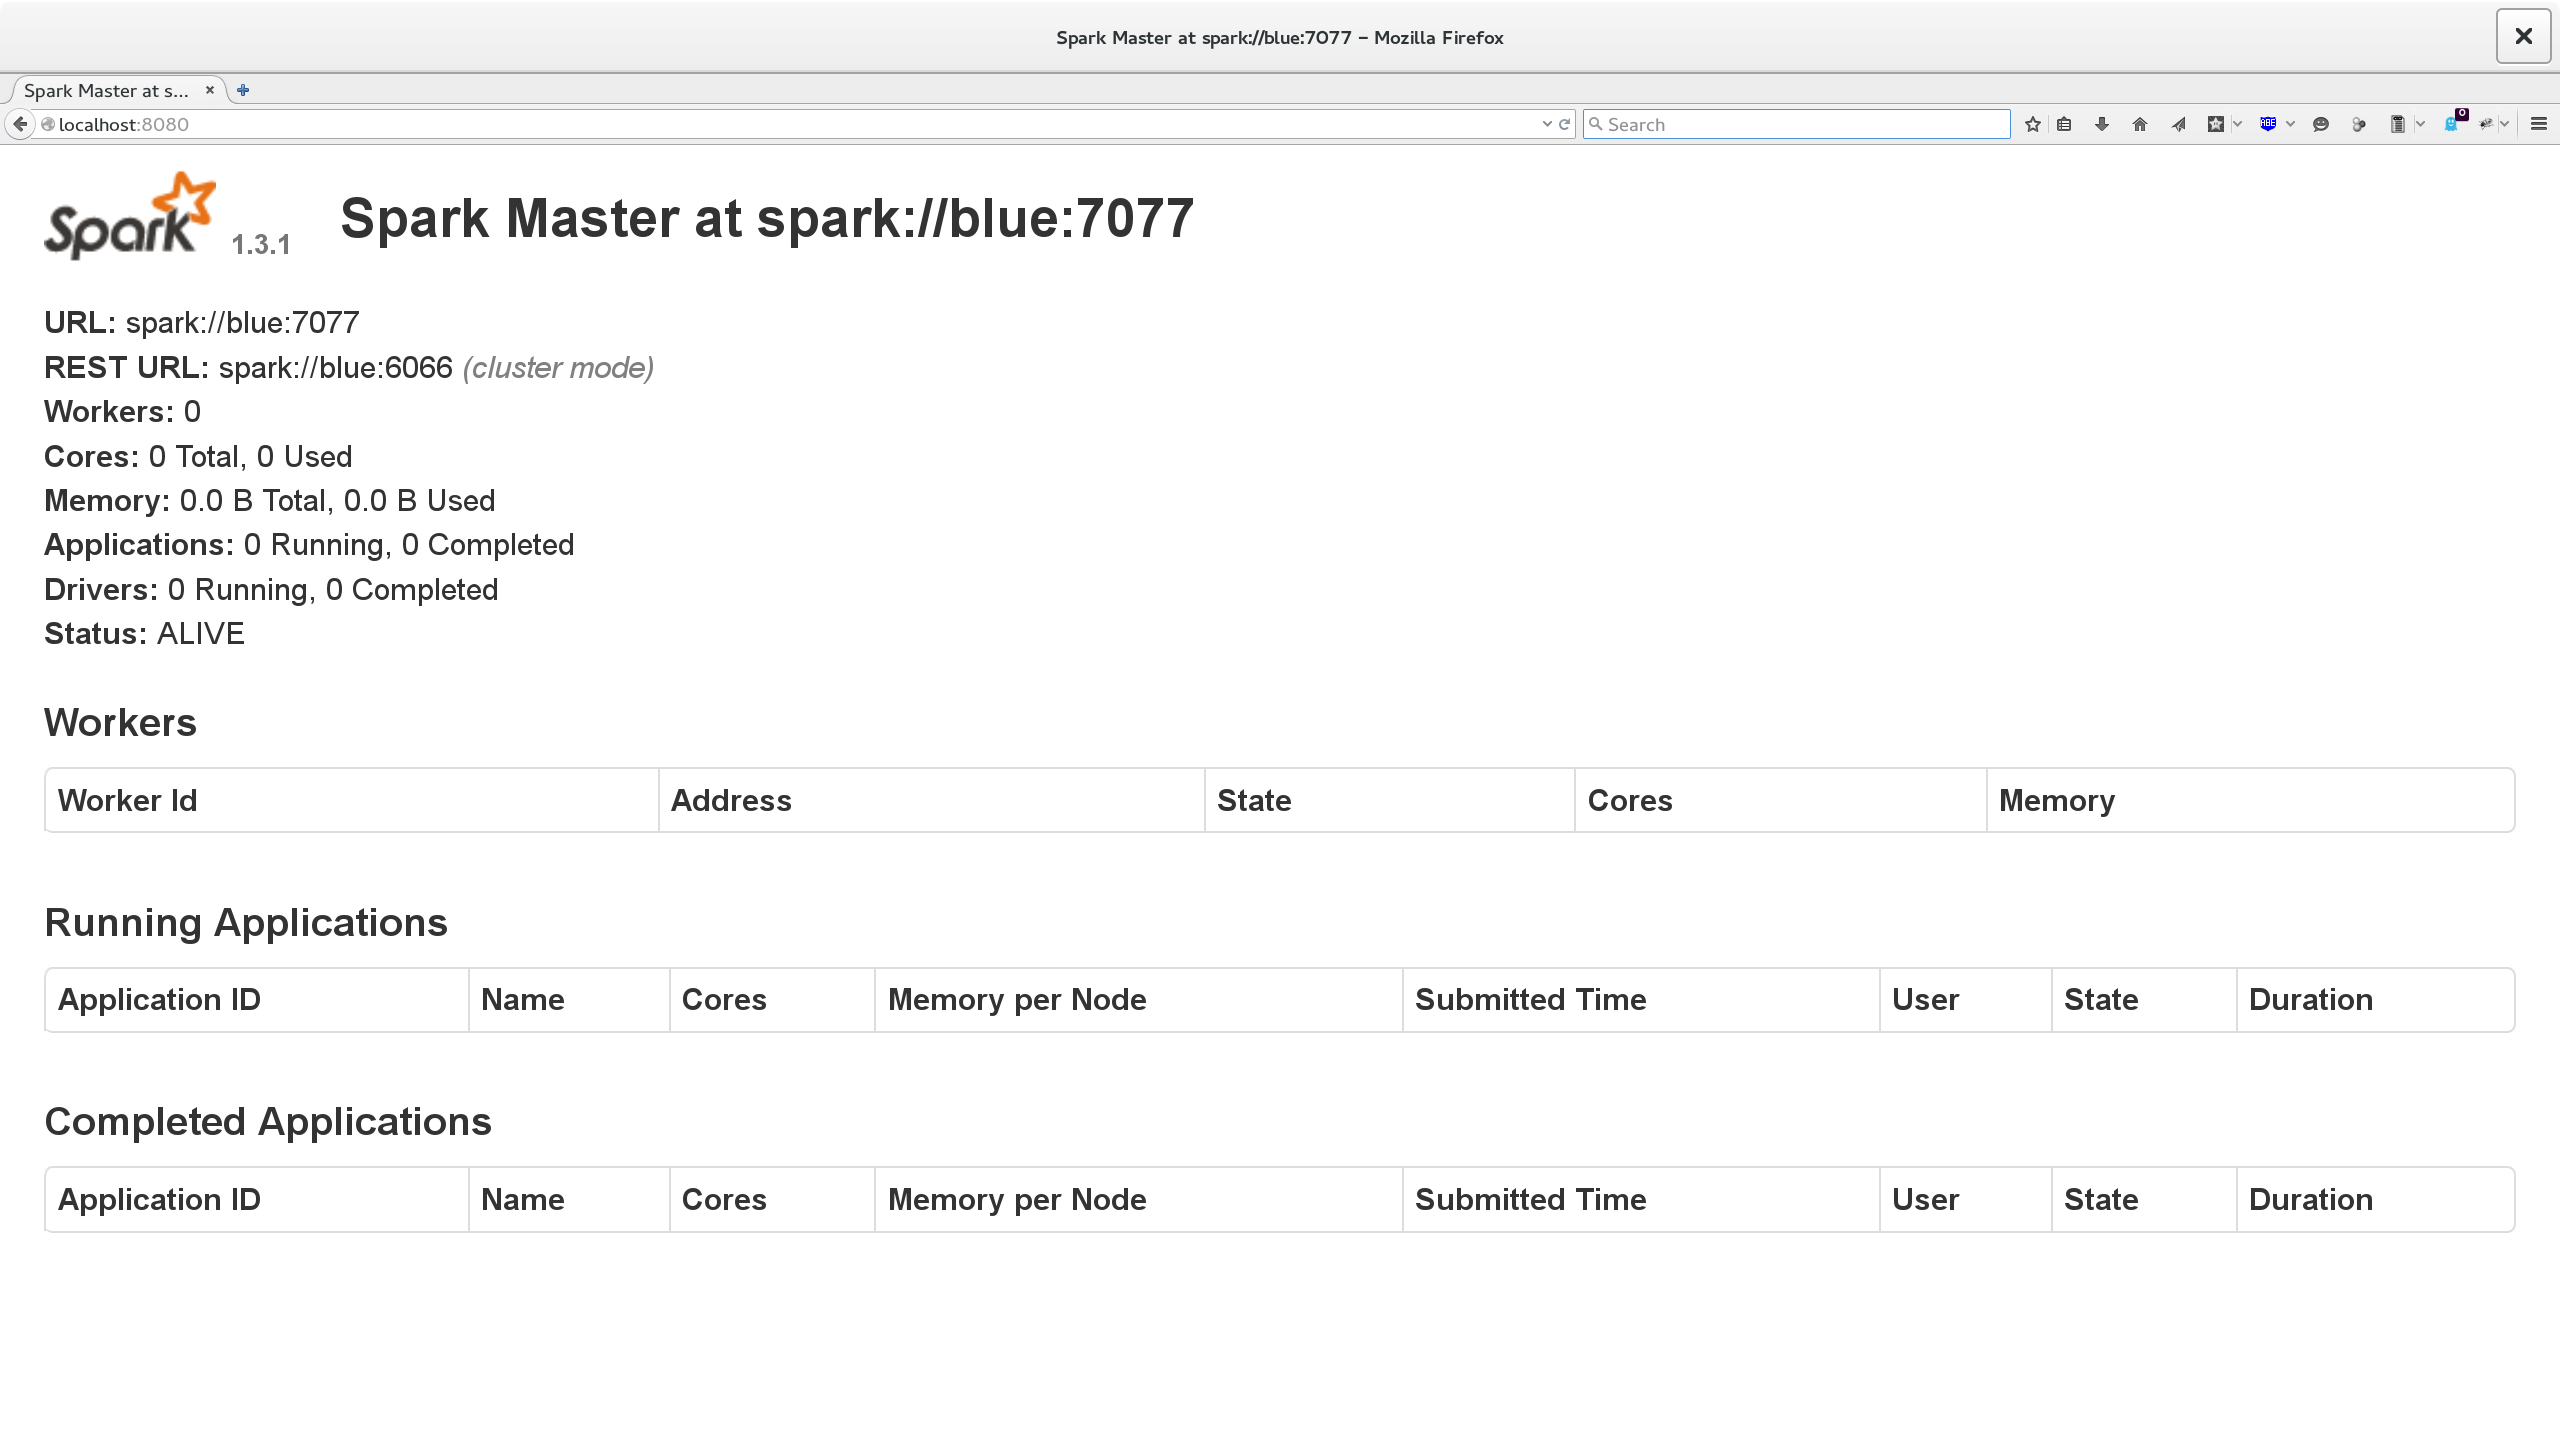
\includegraphics[width=345px]{images/spark_webapp.png}

\end{frame}

%--- EX9 : Launch Worker ---
\begin{frame}[fragile]

  \frametitle{Launch Worker}

  \begin{block}{How To}
    \begin{itemize}
      \item Launch class \textit{org.apache.spark.deploy.worker.Worker} with \textit{spark-class}
      \item With one core : \textit{-c 1}
      \item With 512 Mo of memory : \textit{-m 512M}
      \item Link it to your master : \textit{spark://blue:7077}
      \item Go to localhost:8080
    \end{itemize}
  \end{block}

  \begin{lstlisting}[language=bash, style=terminal-large]
$SPARK_HOME/bin/spark-class \
org.apache.spark.deploy.worker.Worker \
-c 1 \
-m 512M \
spark://blue:7077
  \end{lstlisting} 

\end{frame}

%--- EX9 : Spark Webapp with Worker ---
\begin{frame}

  \frametitle{Spark Webapp with Worker}

  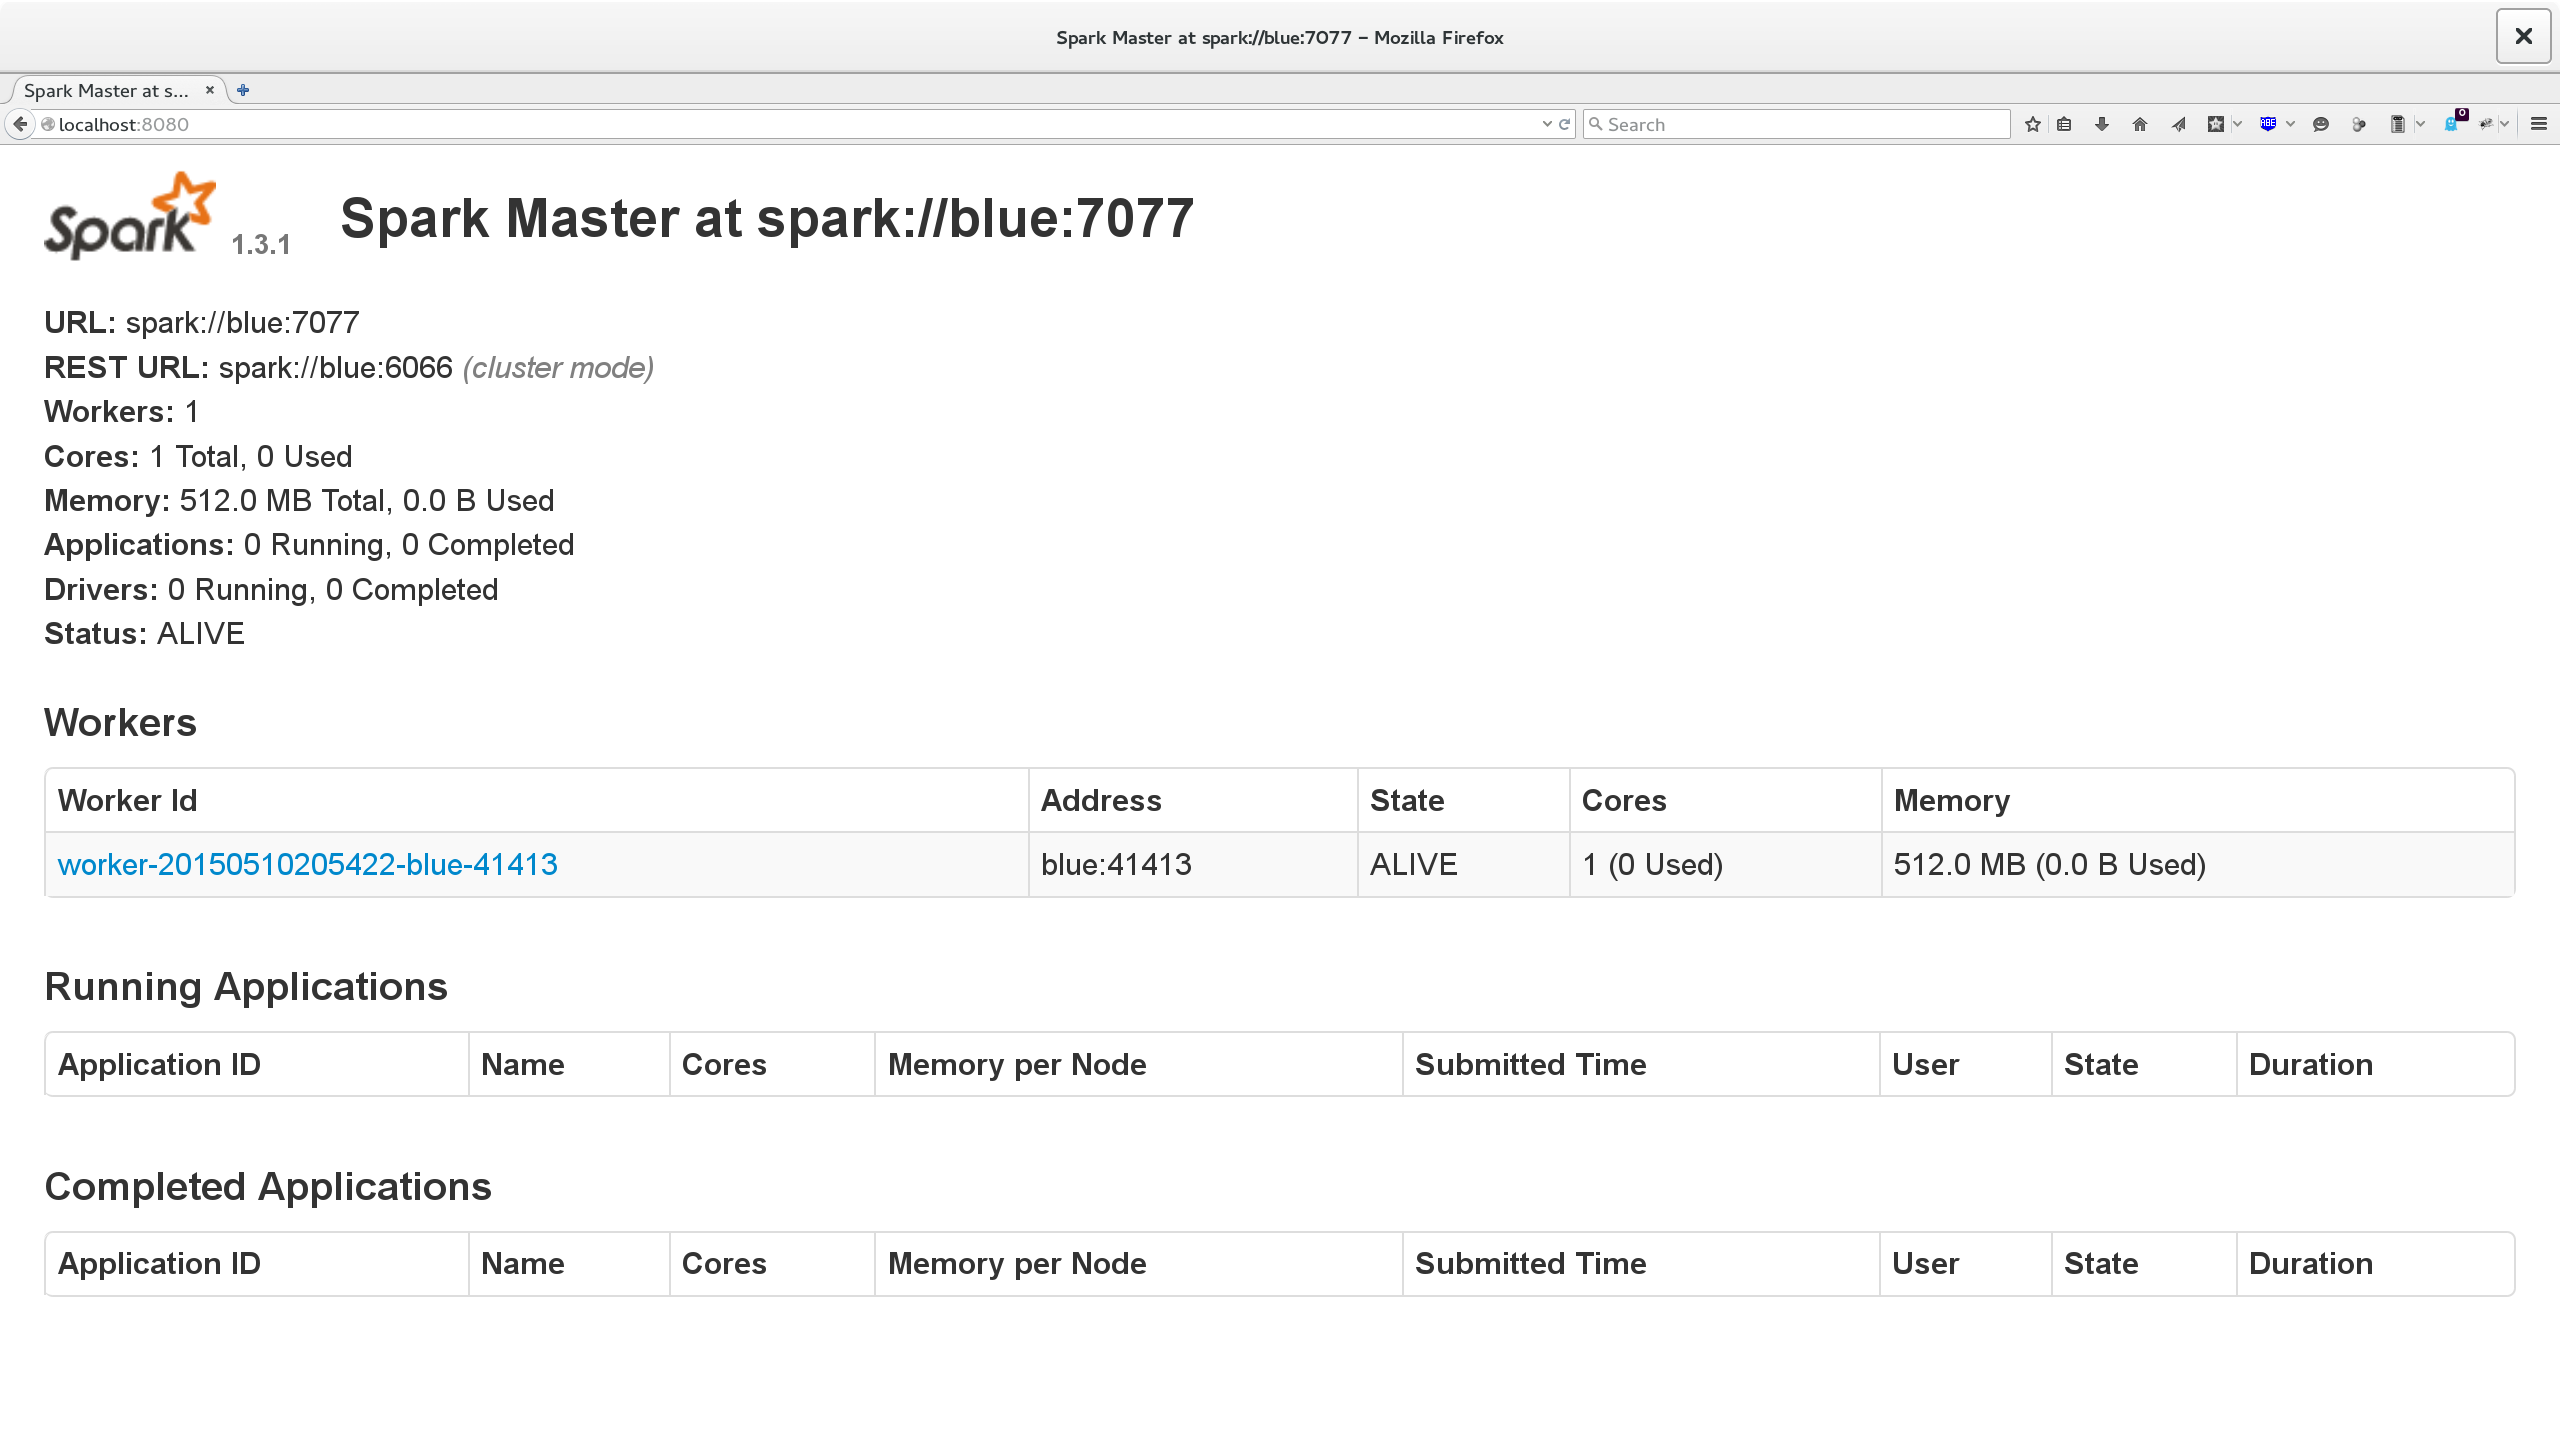
\includegraphics[width=345px]{images/spark_webapp_with_worker.png}

\end{frame}

%--- EX9 : Run Exercise 1 on your cluster ---
\begin{frame}[fragile]

  \frametitle{Run Exercise 1 on your cluster}

  \begin{block}{How To}
    \begin{itemize}
      \item Build project package
      \item Send task to your cluster
      \begin{itemize}
        \item set your master : \textit{--master spark://blue:7077}
        \item set the class you will run : \textit{--class psug.hands.on.solutions.exercise01.SumOfSquaresOfNonPrimeNumbers}
        \item set the deploy mode : \textit{--deploy-mode cluster}
        \item set the package : \textit{target/scala-2.10/psug-hands-on-spark\_2.10-0.0.1.jar}
      \end{itemize}
    \end{itemize}
  \end{block}

  \begin{lstlisting}[language=bash, style=terminal-large]
sbt clean package
$SPARK_HOME/bin/spark-submit \ 
--master spark://blue:7077 \ 
--class psug.hands.on.solutions.exercise01.SumOfSquaresOfNonPrimeNumbers \ 
--deploy-mode cluster \ 
target/scala-2.10/psug-hands-on-spark_2.10-0.0.1.jar
  \end{lstlisting} 

\end{frame}

%--- EX9 : Spark Webapp with a Successful Job ---
\begin{frame}

  \frametitle{Spark Webapp with a Successful Job}

  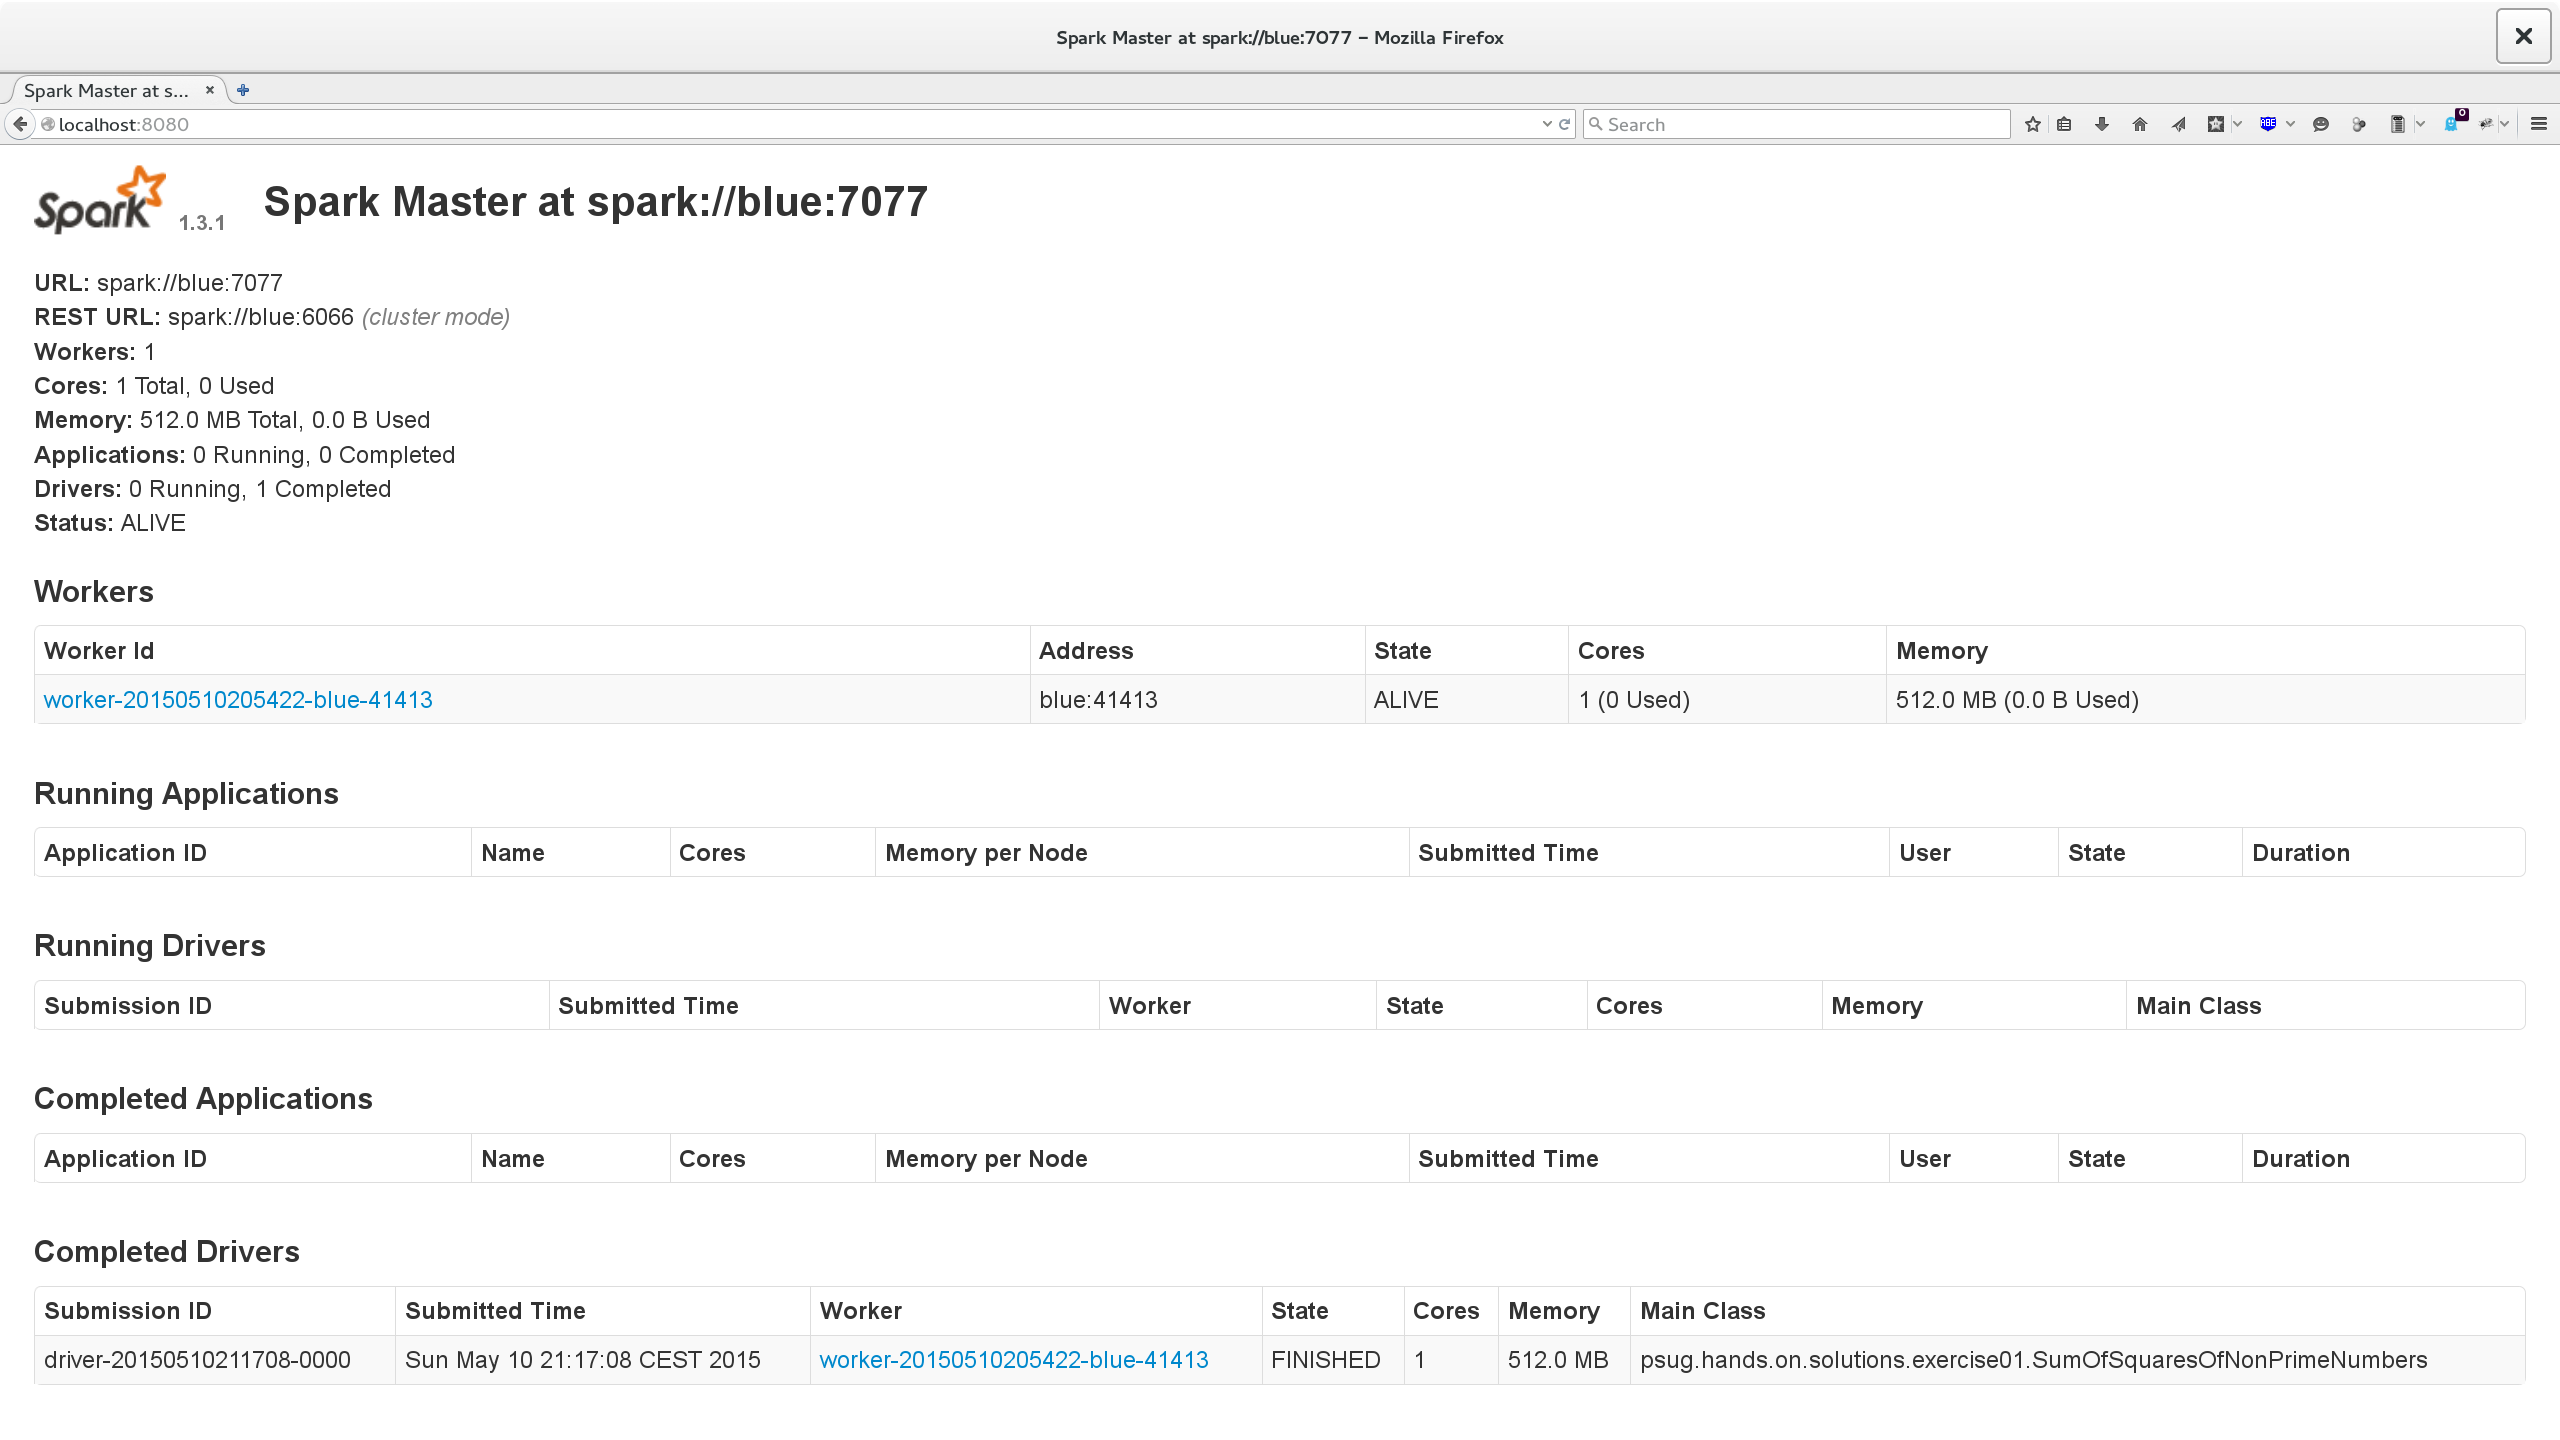
\includegraphics[width=345px]{images/spark_webapp_driver_success.png}

\end{frame}

%--- EX9 : Worker Overview ---
\begin{frame}

  \frametitle{Worker Overview}

  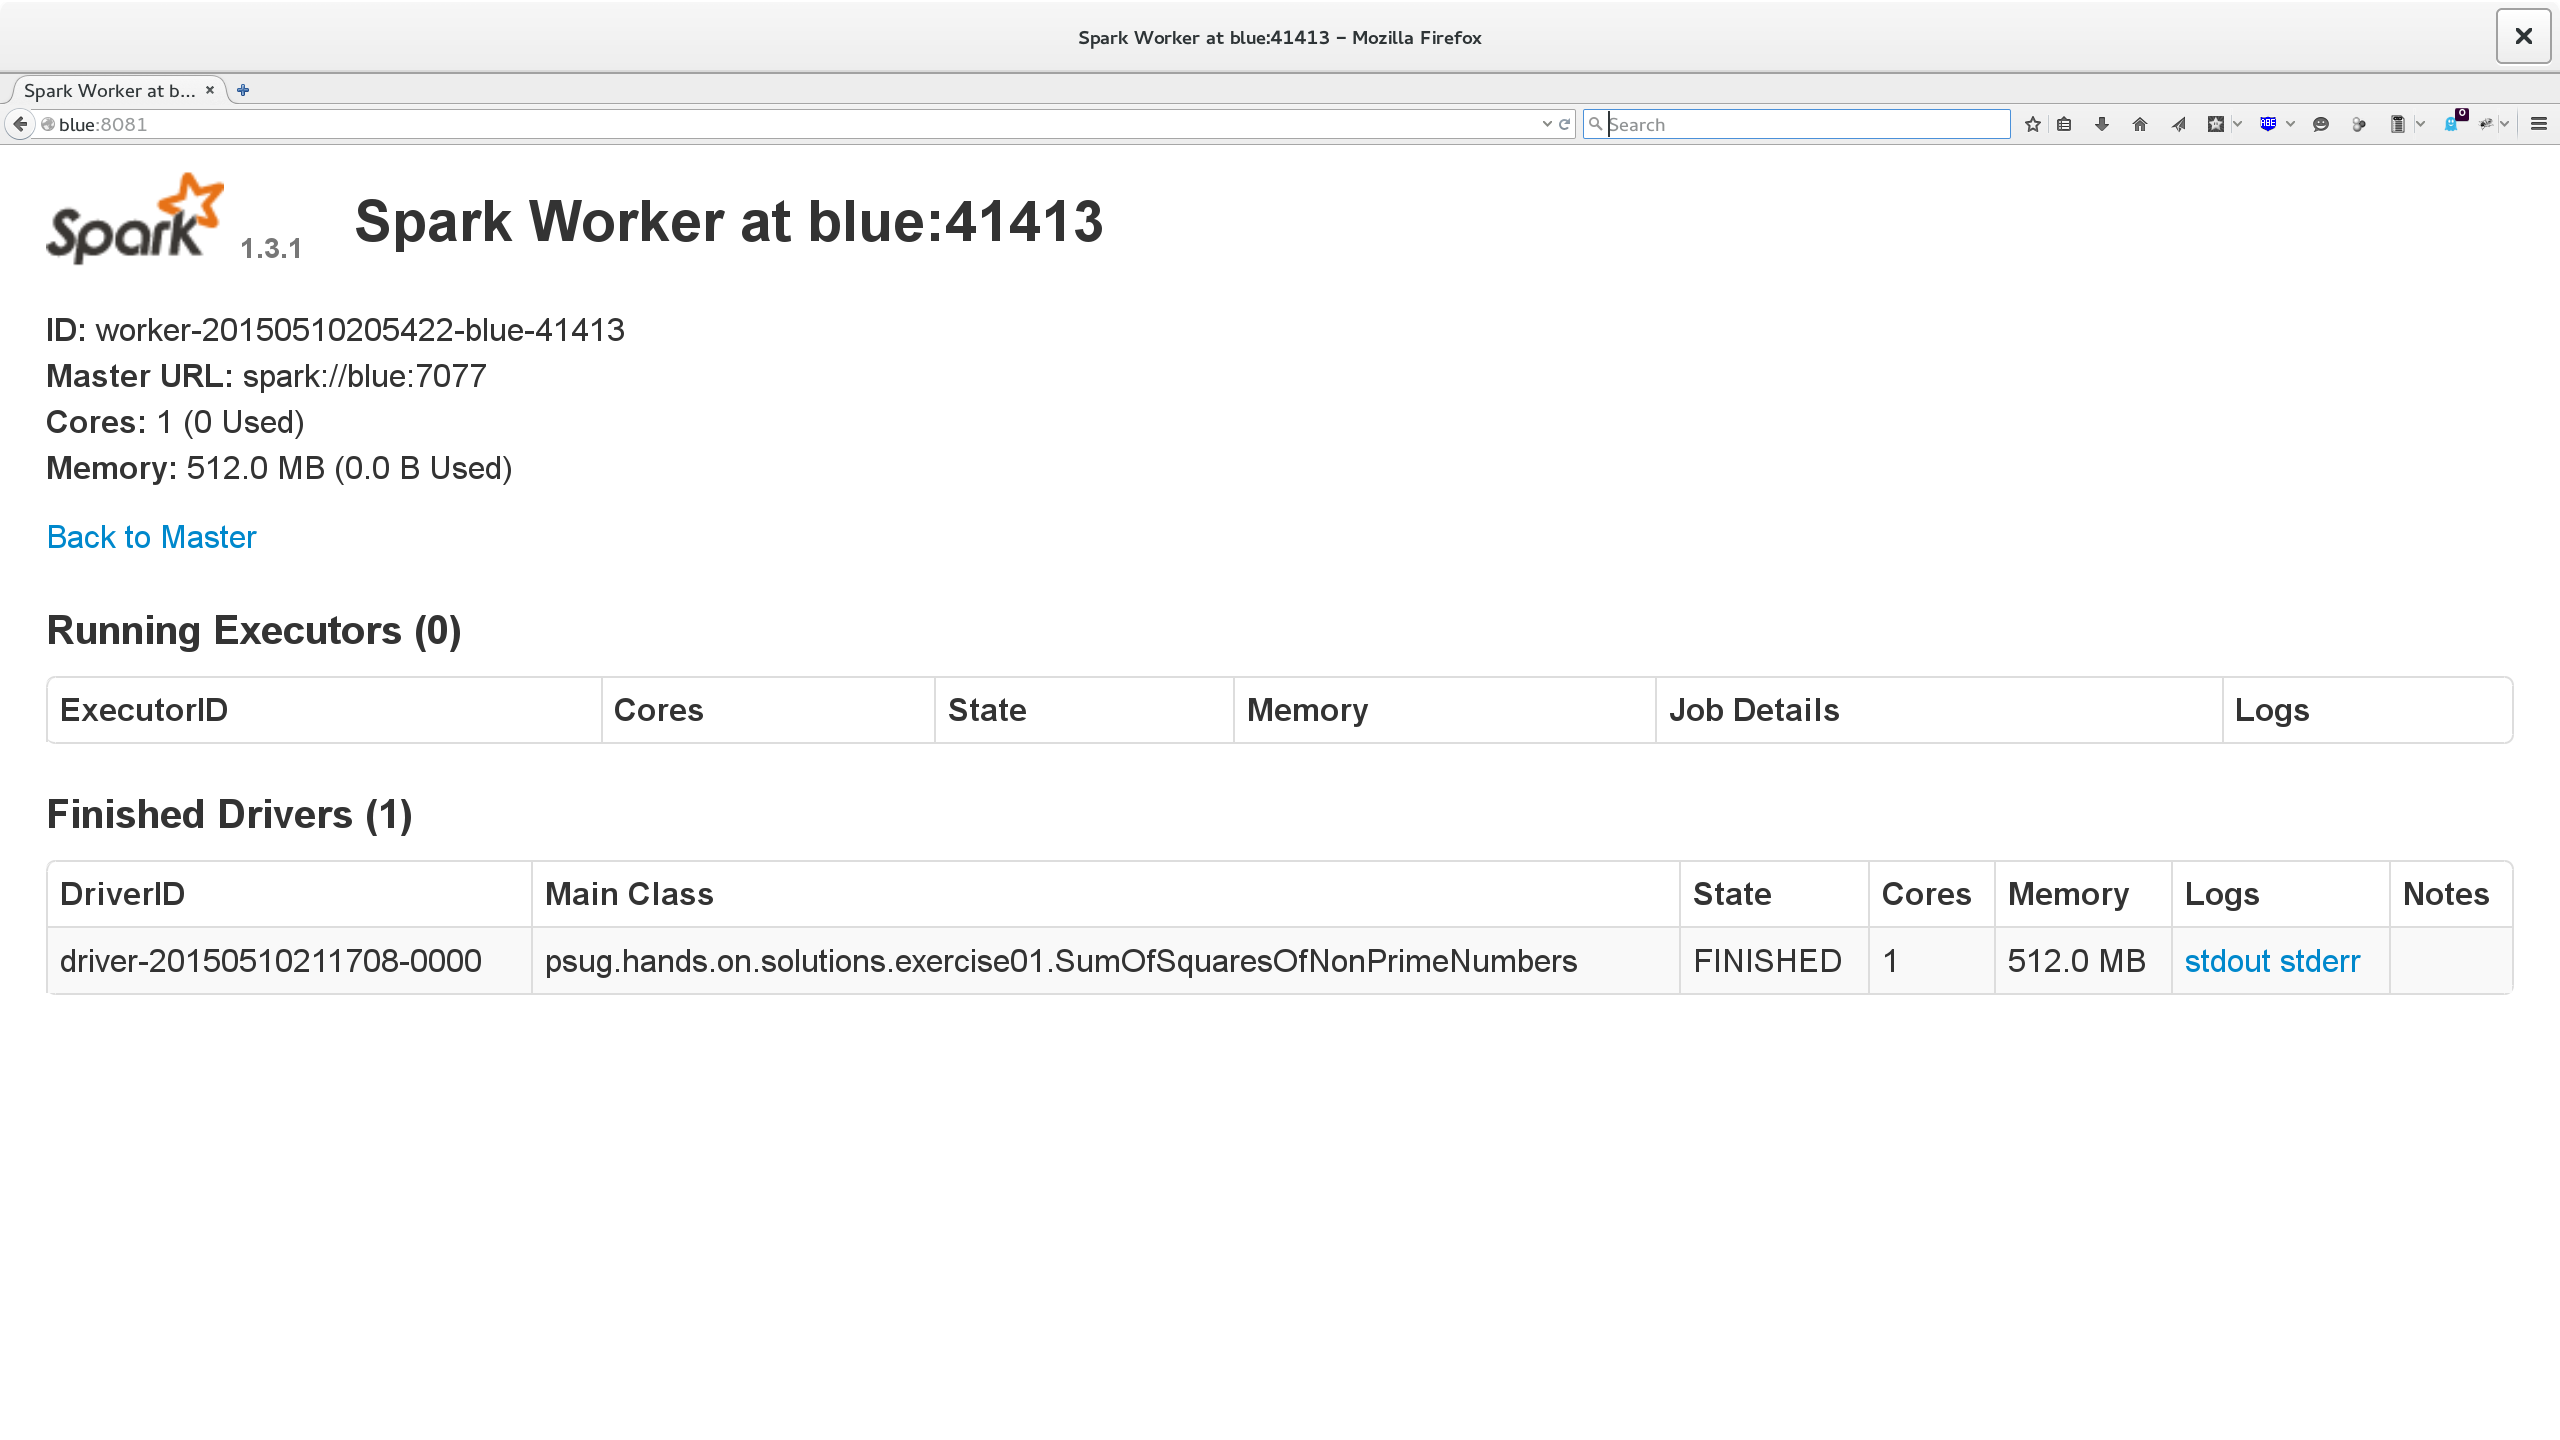
\includegraphics[width=345px]{images/spark_webapp_worker_overview.png}

\end{frame}

%--- EX9 : Worker Logs ---
\begin{frame}

  \frametitle{Worker Logs}

  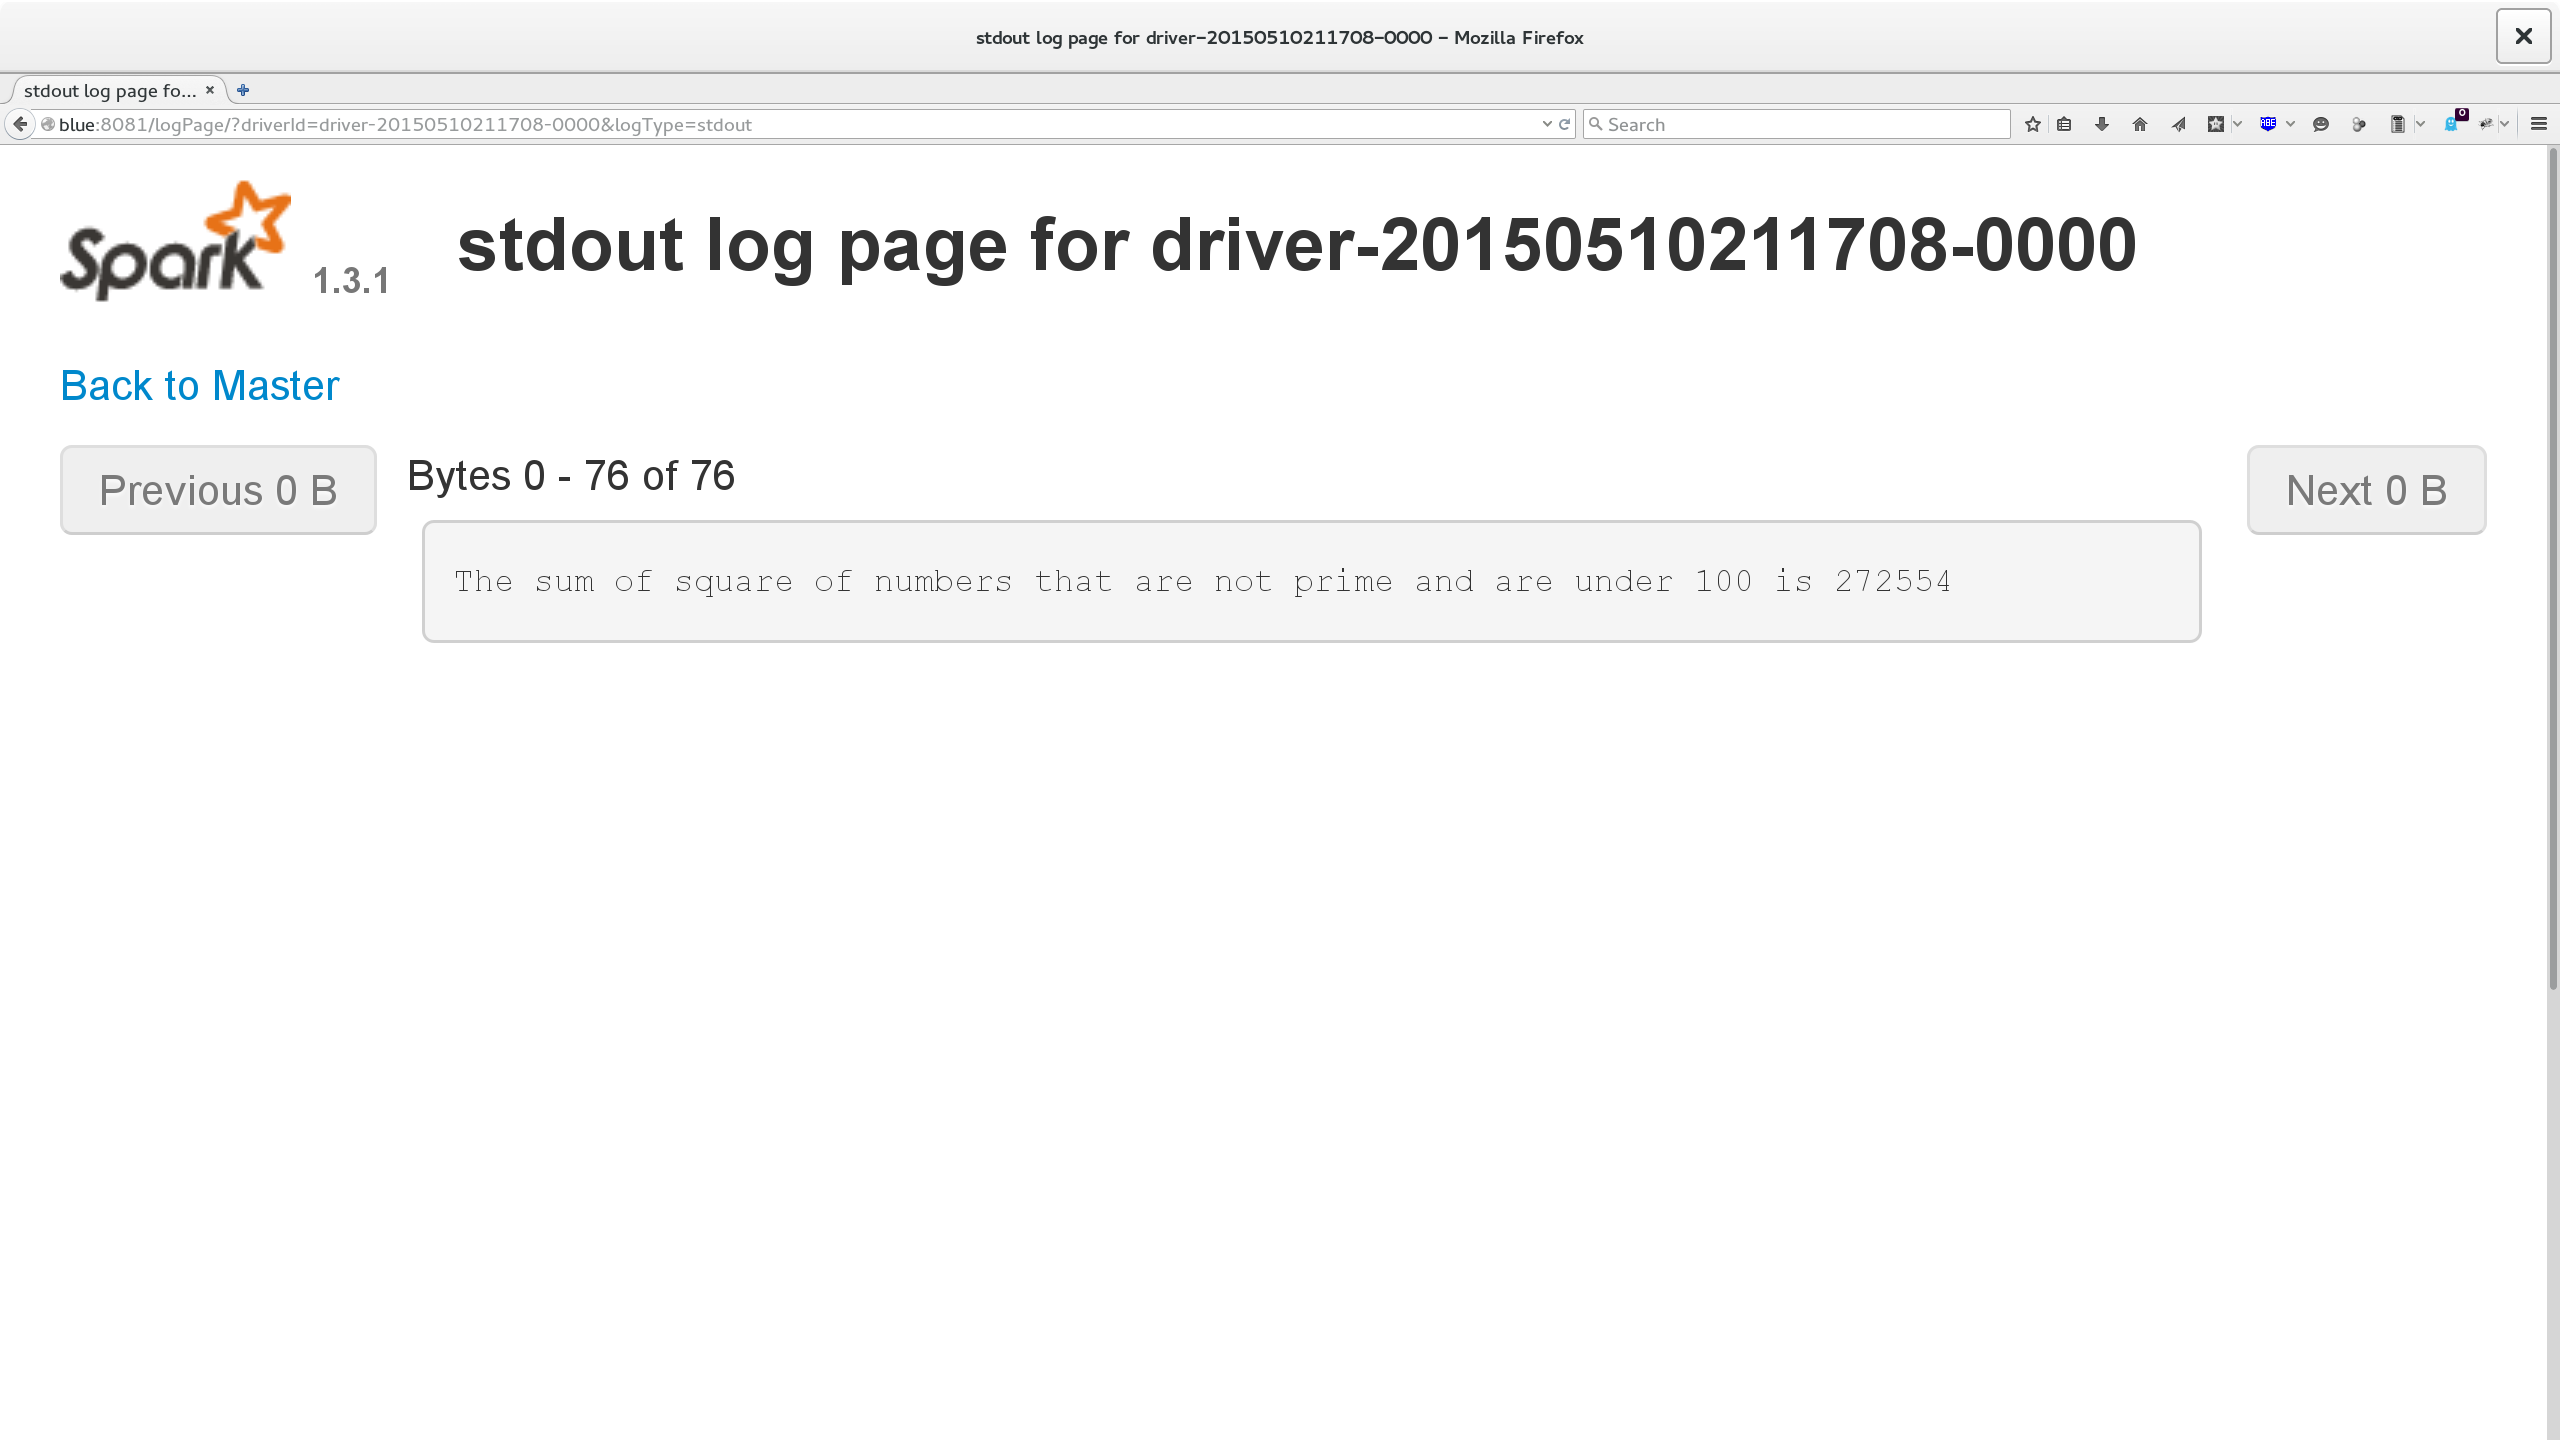
\includegraphics[width=345px]{images/spark_webapp_worker_logs.png}

\end{frame}

%
%
% CONCLUSION
%
%

\section{Conclusion}

%--- What did we do ---
\begin{frame}
  \frametitle{What did we do}

  \Large
  \begin{columns}[T] % align columns
    \begin{column}{.48\textwidth}
      \begin{itemize}
        \item Init Spark Context
        \item Transform List to RDD
        \item Transformations on RDD
        \item Actions on RDD
        \item Stop Spark Context
        \item Load File as RDD
        \item Key/Value RDD
        \item SqlContext and Data Frame
        \item Load JSON as Data Frame
        \item Transform Data Frame to RDD
      \end{itemize}
    \end{column}%

    \hfill%
    \begin{column}{.48\textwidth}
      \begin{itemize}
        \item Drop null value in a Data Frame
        \item Save RDD to JSON File
        \item Perform Sampling
        \item SQL Request on Temporary Tables
        \item Train and use a Machine Learning Model
        \item Launch a Spark Cluster
        \item Submit a task to a Cluster
      \end{itemize}
    \end{column}%
  \end{columns}
  \normalsize
\end{frame}

%--- Transformations and Actions ---
\begin{frame}

  \frametitle{Transformations and Actions}
  
  \LARGE
  \begin{center}
    \begin{tabular}{|c|c|c|c|}
      \hline
      \rowcolor{gray} exercise 1 & exercise 2 & exercise 3 & exercise 4 \\ \hline
      union & filter & \textbf{agg} & \textbf{select} \\
      distinct & flatmap & & \textbf{groupBy} \\
      substract & reduceByKey & & join \\
      map & sortByKey & & sortBy \\ 
       & & & value \\ \hline
      \rowcolor{lightgray} reduce & collect & first & take \\ \hline
      \rowcolor{gray} exercise 5 & exercise 6 & exercise 7 & exercise 8 \\ \hline
      \textbf{where} & & sample & toDF \\
      cache & & & \\ \hline
      \rowcolor{lightgray}   & aggregate & & \\ \hline
    \end{tabular}
  \end{center}
  \normalsize
\end{frame}

%--- Solutions ---
\begin{frame}[fragile]
  \frametitle{Solutions}

  \begin{block}{In your repository}

    \begin{lstlisting}[language=bash, style=terminal-large]
git checkout teacher
git pull
ls src/main/scala/psug/hands/on/solutions 
    \end{lstlisting}
  
  \end{block}

  \begin{block}{On Github}
    https://github.com/vincentdoba/spark-hands-on/tree/teacher/src/main/scala/psug/hands/on/solutions
  \end{block}

\end{frame}

%--- End ---
\begin{frame}

  \frametitle{That's All Folks !}
  
  
  \begin{center}
    \Huge Any Questions ?\normalsize
  \end{center}
\end{frame}


\end{CJK}
\end{document}
